\documentclass[letterpaper]{report}

\usepackage{polyglossia}
\setdefaultlanguage{spanish}



%\usepackage[spanish]{babel}
%\usepackage[utf8]{inputenc}

\usepackage{graphicx}
\usepackage{footnote}
\usepackage{longtable}
\usepackage[top=2.5cm, left=3cm, right=3cm, bottom=2.5cm]{geometry}

\linespread{1.5}

\setlength{\parskip}{2ex}
\parindent 3ex

\usepackage[backend=biber,sorting=none]{biblatex}
\bibliography{Bibliografia/biblio}

\usepackage[linktocpage=true,hidelinks]{hyperref}

\DeclareGraphicsExtensions{.jpg,.pdf,.png}

\begin{document}	
     
     % Portada
%     \begin{titlepage}
    \begin{center}
        
        % Upper part
        
\includegraphics[scale=0.5]{figures/logo} \\
        
        \textsc {\large UNIVERSIDAD SIM\'ON BOL\'IVAR} \\
        \textsc{DECANATO DE ESTUDIOS PROFESIONALES\\
            COORDINACI\'ON DE INGENIER\'IA DE LA COMPUTACI\'ON}
        
        \bigskip
        \bigskip
        \bigskip
        \bigskip
        \bigskip
        \bigskip

        % Aqui coloca el nombre de su proyecto de grado/pasantia larga.
        \textsc{\bfseries HXPLUS OCUPACIONAL.\\
            SISTEMA DE GESTIÓN DE CONSULTAS MÉDICAS\\
             ORIENTADO A MEDICINA OCUPACIONAL}
        
        \bigskip
        \bigskip
        \bigskip
        \bigskip
        \vfill
        
        \begin{minipage}{\textwidth}
            \centering
            Presentado por: \\
            % Aqui coloca su nombre.
            Alejandro Ismael Tarazona López\\
            
            Realizado con la asesoría de:\\
            
            Tutor Académico: Prof. Angela Di Serio\\
            
            Tutor Industrial: Ing. Juan Albarrán\\
            
            \bigskip
            \bigskip
            \vfill
            
            \textbf{INFORME DE PASANTÍA}\\
            
            Presentado ante la Ilustre Universidad Simón Bolívar\\
            
            como requisito parcial para optar por el título de\\
            
            Ingeniero en Computación
            
        \end{minipage}
        
        \bigskip
        \bigskip
        \vfill
        
         {\large \bfseries Sartenejas, julio de 2016}
    \end{center}
        
\end{titlepage}

\pagebreak
     % Título
%     \pagebreak

     
     % Copia y pega
     % Pagina de acta final (vacio)
%     % Pagina del acta final
\begin{titlepage}
    \begin{center}
        
        % Upper part
        
\includegraphics[scale=0.5]{figures/logo} \\
        
        \textsc {\large UNIVERSIDAD SIM\'ON BOL\'IVAR} \\
        \textsc{DECANATO DE ESTUDIOS PROFESIONALES\\
            COORDINACI\'ON DE INGENIER\'IA DE LA COMPUTACI\'ON}
        
        \bigskip
        \bigskip
        \bigskip
        \bigskip
        \bigskip
        \bigskip
        
        % Title
        \textsc{ACTA FINAL PASANTÍA LARGA}
        
        \bigskip
        \bigskip
        
        % Aqui coloca el nombre de su proyecto de grado/pasantia larga.
        \textsc{\bfseries HXPLUS OCUPACIONAL.\\
            SISTEMA DE GESTIÓN DE CONSULTAS MÉDICAS\\
            ORIENTADO A MEDICINA OCUPACIONAL}
        
        \bigskip
        \bigskip
        \bigskip
        \bigskip
        
        \begin{minipage}{\textwidth}
            \centering
            Presentado por: \\
            % Aqui coloca su nombre.
            \textsc{\bfseries Alejandro Ismael Tarazona López} \\
            
            \bigskip
            \bigskip
            \bigskip
            \bigskip
            
            Este Proyecto de Pasantías ha sido aprobado por el siguiente jurado examinador: \\
            
            \bigskip
            \bigskip
            
            % Despues de cada line coloca el (los) nombre(s) de
            % cada uno de los integrantes del jurado.
            \line(1,0){200} \\
            Ángela Di Serio\\
            
            \bigskip
            \bigskip
            
            \line(1,0){200} \\
            Juan Albarrán\\
            
            \bigskip
            \bigskip
            
            \line(1,0){200} \\
            Marlene Goncalves \\
        \end{minipage}
        
        \bigskip
        \bigskip
        \vfill
        
        % Date/Fecha
        {\large \bfseries Sartenejas, julio de 2016}
        
    \end{center}
\end{titlepage}

\pagebreak
     
     \setcounter{secnumdepth}{3}
     \setcounter{tocdepth}{4}
     
     % Define encabezado numeros romanos y como se separan los captiulos y las
     % secciones
     \addtolength{\headheight}{3pt}
     \pagenumbering{roman}
%     \pagestyle{fancyplain}
     
     \renewcommand{\chaptermark}[1]{\markboth{\chaptername\ \thechapter:\,\ #1}{}}
     \renewcommand{\sectionmark}[1]{\markright{\thesection\,\ #1}}
     
%     \onehalfspacing
     
%     \lhead{}
%     \chead{}
%     \rhead{}
%     \renewcommand{\headrulewidth}{0.0pt}
%     \lfoot{}
%     \cfoot{\fancyplain{}{\thepage}}
%     \rfoot{}
     
     % Hasta aquí copié y pege
     
%     	\pagebreak
%     \begin{center}
    \label{dedicatoria}
    A mi padre Augusto.\\
    A mi tío Carlos y a mi abuelo León.\\
    A mi abuela Alicia.\\
    A mis amigos.\\
    A mi amor, Patricia.\\
    \textit{``Dreams come true"}.
\end{center}
\pagebreak
%     \chapter*{Agradecimientos}

Siento que tengo mucho que agradecer pero no hay palabras suficientes para hacerlo.

Primeramente a mi tío Carlos y a mi abuelo León que me han apoyado desde que decidí salir del nido, sin su apoyo y sus consejos no estaría acá.

A mi papá, gracias por estar ahí en mis tormentas y por esas semillas de sabiduría que me diste. Gracias desde el fondo de mi corazón.

A Patricia, gracias por ser mi calma y compañía.

A mis amigos por estar ahí para escucharme y poder drenar las rabietas o frustraciones de cada trimestre y celebrar los logros también. ¡Salud!

\pagebreak
     
     \tableofcontents
     
     % Índice de figuras
     % Crea la lista de cuadros
     \listoftables
     
     % Crea la lista de figuras
     \listoffigures
     
     % Crea la lista de codigos fuentes
     %\lstlistoflistings
     
%     \clearpage
     
     % Lista de acrónimos y abreviaturas
     \chapter*{Lista de Abreviaturas}
\begin{table*}[h!]
    \begin{center}
        \begin{tabular}{ll}
            \textbf{API} & Application Programming Interface\\
            \textbf{DI} & Demendency Inyection\\
            \textbf{ECMA} & European Computer Manufacturers Asociation\\
            \textbf{GPL} & General Public Licence\\
            \textbf{HTML} & Hypertext Modeling Language\\
            \textbf{HTTP} & Hypertext Transfer Protocol\\
            \textbf{IOC} & Inversion Of Control\\
            \textbf{JPA} & Java Persistence API\\
            \textbf{JS} & JavaScript\\
            \textbf{JSON} & JavaScript Object Notation\\
            \textbf{LAMP} & Linux Apache MySQL PHP (Perl o Python)\\
            \textbf{MVC} & Modelo Vista Controlador\\
            \textbf{PDF} & Portable Document Format\\
            \textbf{POJO} & Plain Old Java Object\\
            \textbf{POM} & Project Object Model\\
            \textbf{SOA} & Service Oriented Architecture\\
            \textbf{SQL} & Structured Query Language\\
            \textbf{UI} & User Interface\\
            \textbf{USB} & Universal Serial Bus\\
        \end{tabular}
    \end{center}
\end{table*}
     
     % Define encabezado en numeros arabicos  
     \pagenumbering{arabic}
     
     % Lista de símbolos y abreviaturas
     \chapter*{Introducción}
\addcontentsline{toc}{chapter}{Introducción}
\pagebreak
     \chapter{Entorno Empresarial}

En el presente capítulo se describe el entorno en el cual se desarrolló el proyecto de pasantía HxPlus Ocupacional, el cual fue realizado para la empresa Globinsoft S.A. Se presenta la historia, descripción, estructura organizacional y el cargo ocupado por el pasante dentro de la misma.

    \section{Antecedentes}
    
    Globinsoft S.A. es una empresa destinada a prestar servicios en el área médica, brindado herramientas y soporte con la finalidad de facilitar, tanto a médicos y asistentes como a pacientes, el acceso a la información sobre las historias médicas, en caso de los pacientes sólo a su historia personal.
    
    Globinsoft S.A. posee en la actualidad su producto ``HxPlus" el cual tiene como objetivo el almacenamiento de historias médicas de manera digital, usando tecnología web, para mantener su disponibilidad a cualquier hora del día y desde cualquier dispositivo con acceso a la web. Cuenta también con la opción de generar informes médicos, récipes y reposos médicos para uso de los farmacéutas y comodidad de los pacientes.
    
    
    \section{Misión}
    
    Brindar apoyo tecnológico al área médica en Venezuela, prestando servicios de calidad dentro del marco de lo estipulado por el Ministerio de Salud.
    
    \section{Visión}
    
    Ofrecer una plataforma integral para la gestión de consultas, historias médicas, récipes y medicamentos con alcance nacional y disponibilidad las 24 horas del día, los 7 días de la semana.
    
    \section{Estructura organizacional}
    
    Globinsoft S.A. mantiene los siguientes departamentos:
    
    \begin{enumerate}
        \item Gerencia.
        \item Recursos Humanos.
        \item Finanzas y Contabilidad.
        \item Proyectos.
    \end{enumerate}
    
    En la gerencia de proyectos se ubica el ingeniero Juán Albarrán, quien a su vez tiene el papel de tutor industrial de la pasantía descrita en el presente informe. La gerencia de proyectos se divide en cada uno de los proyectos realizados por la empresa y hasta el momento de la presente redacción, se cuenta con ``HxPlus" como proyecto en producción, al cual se le hace seguimiento, y soporte, y ``HxPlus Ocupacional" como proyecto en desarrollo. Figura \ref{estructura-org}.
    
    \begin{figure}[htbp!]
        \begin{center}
            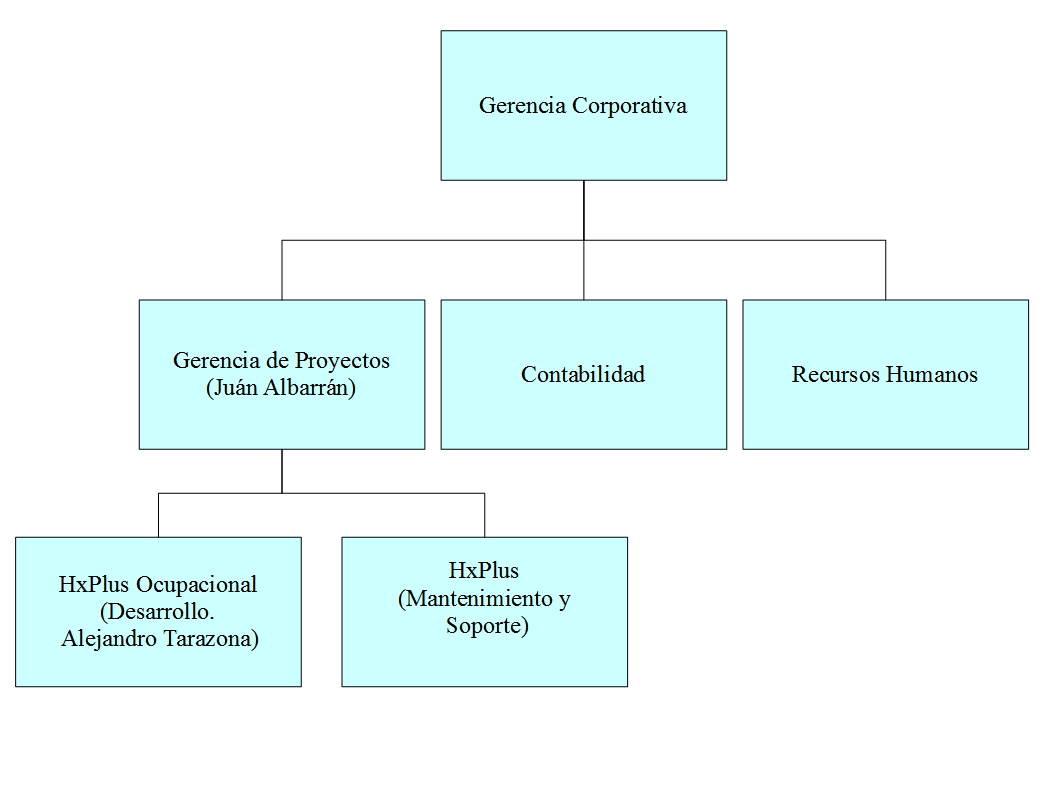
\includegraphics[scale=.25]{figures/Estructura}
        \end{center}
        \caption{Estructura Organizacional de Globinsoft}
        \label{estructura-org}
    \end{figure}

\pagebreak
     \chapter{Marco Teórico}

En el presente capítulo se describen conceptos y patrones utilizados para el desarrollo del proyecto de patantía, los cuales fueron seleccionados siguiendo los criterios de usabilidad, mantenibilidad, escalabilidad y portabilidad.

    \section{Modelo Vista Controlador (MVC)}
    
    El Modelo-Vista-Controlador es un patrón de arquitectura de \textit{software} que separa el modelo (Objetos de negocio) la vista (Interfaz con el usuario u otros sistemas) y el controlador (Manejo de la informacion de negocio)\cite{MVC-tiw}.
    
    Específicamente, cada componente tiene una asignación independiente de los demás componentes. Estas son:
    
    \begin{enumerate}
        \item \textbf{Modelo}
            \begin{itemize}
                \item Almacenamiento de los datos.
                \item Estado de la aplicación.
                \item Recuperación de errores en los datos.
            \end{itemize}
        \item \textbf{Vista}
            \begin{itemize}
                \item Presentación del modelo.
                \item Puede acceder al modelo pero no cambiar su estado.
            \end{itemize}
        \item \textbf{Controlador}
            \begin{itemize}
                \item Reaccionar a las peticiones del cliente.
                \item Comunicar al modelo de las acciones ejecutadas.
                \item Direccionar a las vistas requeridas del lado del cliente.
            \end{itemize}
    \end{enumerate}
    
    \section{Arquitectura Orientada a Servicios(SOA por sus siglas en inglés, \textit{Service Oriented Architecture})}
    
    A parte del patrón MVC que garantiza el bajo acoplamiento del sistema, se tiene la filosofía de desarrollo orientada a servicios la cual actúa como una guía de desarrollo y facilita el mismo orientado a la escalabilidad del sistema, esto es: facilita las actializaciones de alguno de los componentes MVC y minimiza el efecto que dicha actualización tiene sobre los demás.
    
    Según Gartner\cite{SOA-libroGartner} y González Quiroga\cite{SOA-tesis}, la incorporación de SOA empieza en las empresas hacia 2003, por las siguiente razones:
    
    \begin{itemize}
        \item La incesante presión de los negocios para la agilidad. Cuando una empresa quiere
        modificar sus procesos, productos o servicios, no puede permitirse el lujo de esperar por
        mucho tiempo. Debe ser posible cambiar la forma de aplicación de los sistemas de
        trabajo simplemente modificando los componentes que ya están en uso, en lugar de
        comprar o codificar nuevos componentes o sistemas enteros desde cero.
        
        \item La flexibilidad de la arquitectura SOA basada en Servicios Web de apoyo a múltiples
        aplicaciones.
        
        \item  La aceptación unánime de proveedores de los estándares de Servicios Web,
        especialmente de Simple Object Access Protocol (SOAP) y Web Service Description
        Language (WSDL)\cite{SOA-libroGartner}
        
    \end{itemize}
    
    SOA se basa en capas, cada una servicios a la siguiente y sus procedimientos internos se mantienen ocultos a las demás capas. Con esto se generan APIs de acceso estandarizado y son independientes de las tecnologías utilizadas en el desarrollo.
    
    En \textit{Service Oriented Architecture}\cite{SOA-msdn} definen SOA usando el poema de Saxe sobre los ciegos y el elfante.
    
    "Seis ciegos de Indostan se encuentran con un elefante, cada uno describe el elefante de forma diferente porque se ve influenciado por sus propias experiencias
    
    \begin{itemize}
        \item Quien le toca la trompa cree que es una serpiente.
        \item Quien le toca los colmillos cree que son lanzas.
        \item Quien le toca las orejas cree que son abanicos.
        \item Quien le toca la panza cree que es una pared.
        \item Quien le toca la cola cree que es una cuerda.
        \item Quien le toca	las patas cree que son árboles."
    \end{itemize}
    

    \begin{figure}
        \begin{center}
            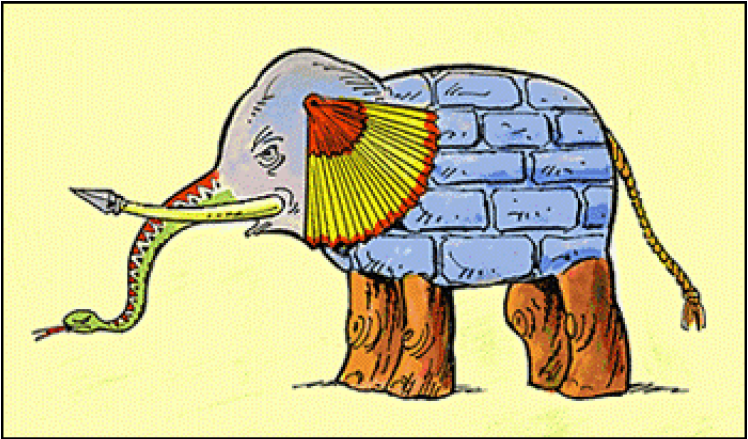
\includegraphics[scale=.75]{figures/Elefante}
        \end{center}
        \caption {El elefante de Saxe}
    \end{figure}

    Se usa la analogía para ejemplificar el hecho de que haya varias definiciones diferentes de lo que es SOA en si, porque se le ha definido como patrón de diseño o como una filosifía de desarrollo, siendo esta última la definición adoptada para el trabajo descrito en el presente informe.
    
    También se puede usar dicha analogía para ejemplificar cómo las (potenciamente) distintas vistas pueden interactuar con el controlador y este a su vez con el modelo.


    \section{Autenticación Basada en \textit{Tokens}}
    
    Es una forma de autenticación ligera\cite{ToTOKEN-tokenbasedauth}, que va de la mano con SOA, que usa \textit{tokens} o fichas cifradas para la verificación de usuarios. Estas fichas son almacenadas en el cliente y enviadas en cada una de los \textit{requests} que realiza el navegador, la ficha es decifrada y se verifican las credenciales del usuario en cuestión.
    
    Entre los datos almacenados en las fichas están:
    
    \begin{itemize}
        \item Nombre de usuario.
        \item Fecha de autenticación.
        \item Fecha de caducidad de la ficha.
    \end{itemize}
    
    Estas son cifradas en el servidor bajo una clave secreta elegida por el mismo servidor y que se usa para el posterior decifrado de las fichas.
    
    Todo esto permite que el servidor no se sobrecargue con variables de estado o de sesión por cada usuario autenticado en un momento dado y además permite la portabilidad desesada para el sistema.
    
\pagebreak
     \chapter{Marco Metodológico}

    En el presente capítulo se describe la metodología usada para el desarrollo del proyecto así como sus componentes, los actores que participaron y los roles que cumplieron en el desarrollo del mismo.

    Para \textit{HxPlus Ocupacional} fue seleccionado Scrum como metodología de desarrollo a seguir. Y aunque no está estipulado por la metodología, se llevaron a cabo diagramas de casos de uso y de clases para una documentación completa del sistema.
    
    Scrum es una metodología de gestión de proyectos ágil que utiliza uno o más equipos de trabajo, de a lo sumo 7 personas, en iteraciones de tiempo fijo, llamados \textit{Sprints}, para la entrega de tareas o avances en el proyecto que sean funcionales y probados
    \footnote{Con información de \citeauthor{scrum-guia}\cite{scrum-guia}, \citeauthor{scrum-primer}\cite{scrum-primer} y \citeauthor{scrum-agile}\cite{scrum-agile}}.    
    
    Los equipos apuntan siempre a conseguir avances limpios, probados y aceptados de manera que puedan ser puestos en producción inmediatamente.
    
    Scrum se divide en Roles, Eventos y Artefactos tal como se describe a continuación:

    \section{Roles}
        
        \subsection{Product Owner}
        \label{product-owner}
        
        Este rol representa la voz del cliente en la gestión del proyecto. Debe velar por la realización del proyecto desde la perspectiva del negocio. Se encarga de escribir las historias de usuario, las prioriza y las anexa al ``Product Balcklog" (o también Lista del Producto).
        
        El Dueño de Producto es la única persona responsable de gestionar la Lista del Producto. La gestión de dicha lista, según expresa \citeauthor{scrum-guia}\cite{scrum-guia}, consiste en:
        
        \begin{itemize}
            \item Expresar claramente los elementos de la Lista del Producto.
            \item Ordenar los elementos en la Lista del Producto para alcanzar los objetivos y misiones de la mejor manera posible.
            \item Optimizar el valor del trabajo desempeñado por el Equipo de Desarrollo.
            \item Asegurar que la Lista del Producto es visible, transparente y clara para todos, y que muestra aquello en lo que el equipo trabajará a continuación.
            \item Asegurar que el Equipo de Desarrollo entiende los elementos de la Lista del Producto al nivel necesario.
        \end{itemize}
               
        Para el presente proyecto se designó al ingeniero Juan Albarrán como Product Owner siendo el mejor representante de los intereses de Soluciones Globinsoft S.A. y estando él familiarizado tanto con los porcesos de negocio como con el equipo de desarrollo y el proceso de desarrollo mismo.
        
        \subsection{Scrum Master}
        \label{scrum-master}
        
        Es el responsable de llevar el procedimiento de gestión del proyecto según los lineamientos de Scrum. Sirve de asesoría entre invloucrados y comprometidos en materia de organización y distribución de la información. Él dirige las reuniones y vela por su cumplimiento según las reglas de procedimiento de Scrum.
        
        \citeauthor{scrum-guia}\cite{scrum-guia} clasifica los servicios del Scrum Master en tres categorías:
        \begin{enumerate}
            \item Servicio al dueño del producto
            \begin{itemize}
                \item Asesoramiento para la gestión eficiente de la Lista del Producto.
                \item Asesoramiento para la planificación del producto.
            \end{itemize}
            
            \item Servicio al equipo de desarrollo
            \begin{itemize}
                \item Apoyar en la organización del equipo.
                \item Eliminar los impedimientos y dificultades que limiten el progreso del equipo.
                \item Facilitar la organización de los eventos de Scrum según sea requerido.
                \item Guiar al equipo en entornos donde Scrum no haya sido del todo adoptado.
                \item Apoyar al equipo en dudas que surjan respecto a los eventos y artefactos de Scrum.
            \end{itemize}
            \item Servicio a la organización
            \begin{itemize}
                \item Liderar la adopción de Scrum como metodología de desarrollo.
                \item Asesorar a los empleados en el uso de Scrum y sus procedimientos.
            \end{itemize}
        \end{enumerate}
        
       Por su experiencia en previos proyectos, entre ellos \textit{HxPlus} (antecedente de \textit{HxPlus Ocupacional}) y su amplio conocimiento en el negocio, se le delegó también el puesto de ``Scrum Master" en el presente proyecto al ingeniero Juan Albarrán.
        
        \subsection{Development Team}
        \label{development-team}
        
        Es el conjunto de personas dedicadas a construir el producto indicado por el dueño del producto. Se requieren que sean grupos lo suficientemente pequeños como para fomentar un alto nivel de independencia y autoorganización pero, a su vez, lo suficientemente grandes como para poder presentar avances significativos en cada Sprint y que potencialmente, estos avances, puedan ser puestos en producción.
        
        Equipos pequeños, de menos de tres personas, reduce la productividad global y reduce los posibles avances en el producto. También podrían presentar limitaciones en cuando a las habilidades de los integrantes, lo cual resultaría convirtiéndose en impedimentos en el desarrollo.
        
        Por otro lado, equipos muy grandes, de más de nueve miembros requiere demasiada coordinación entre los miembros lo cual podría significar una menor eficiciencia y mayor trabajo para la organización de los avances. En otras palabras, se perdería agilidad tratando de organizar un equipo semejante.
        
        Idealmente un equipo de desarrollo varía entre tres y siete personas. Esto mantiene un equilibrio saludable entre la cantidad de trabajo que pueden manejar y la capacidad de autoorganización del equipo.
        
        El equipo debe ser multifuncional, debe tener las capacidades necesarias para desarrollar el producto y poder apoyarse entre sí para compensar los puntos débiles de cada individuo.
        
        No existen roles dentro del equipo de desarrollo. A pesar que uno podría desempeñarse mejor en un área de desarrollo, no existen como tal roles. Esto es debido a que la responsabilidad del desarrollo recae sobre el equipo como un todo y sobre ningún miembro en particular, por ello tampoco existe un rol de Líder o Jefe de Proyecto.
        
        Para HxPlus Ocupacional el equipo de desarrollo consta de un solo miembro, Alejandro Tarazona, pasante y autor del presente libro.
        
    \section{Eventos}
    
    Esta sección describe los eventos determinados por la metodología seleccionada y cómo fueron establecidos para la gestión del proyecto. Estos son:
    
    \begin{figure}[htbp!]
        \begin{center}
            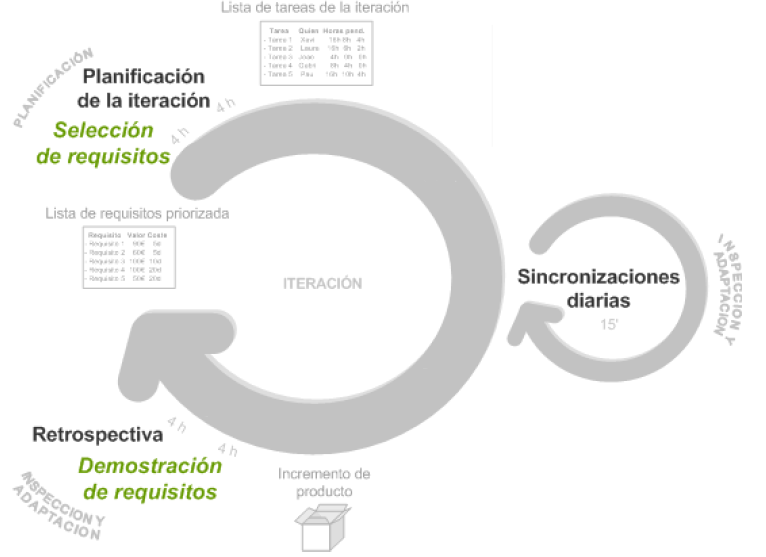
\includegraphics[width=.8\textwidth]{figures/scrum}
        \end{center}
        \caption{Esquema de trabajo de SCRUM}
        \label{scrum-esquema}
    \end{figure}
    
        \subsection{Sprint}
        
        Unidad mínima de desarrollo, usualmente determinada por una tarea corta o un período de tiempo pequeño, usualmente 1 o 2 semanas, nunca más de 30 días; durante el cual el equipo de desarrollo trabaja según las metas estipuladas al principio del mismo. Normalmente éstas metas no cambian durante el desarrollo del Sprint sino al final del mismo, cuando se planifica el siguiente Sprint.
        
        Para HxPlus Ocupacional fue determinado en una semana para las primeras tareas y dos para las últimas, debido a las pruebas subyacentes y el trabajo de integración que representan.
        
        Se llevaron a cabo 3 fases:
        \begin{enumerate}
            \item Preparación (1 Sprint)
            \item Desarrollo (8 Sprints)
            \item Cierre (2 Sprint)
        \end{enumerate}
        
        Tal y como se describe en el capítulo \ref{desarrollo-capitulo}.
        
        \subsection{Sprint Planning}
        
        Planificación del siguiente Sprint a realizar. El equipo de desarrollo (``Development Team", punto \ref{development-team}) hace los pronósticos e indica qué puede llevar a cabo en el siguiente Sprint de lo que propone el dueño del producto (``Product Owner", punto \ref{product-owner}) que debe hacerse durante el Sprint. El ``Scrum Master" (punto \ref{scrum-master}) está encargado de revisar cuidadosamente con el equipo las posibilidades, negociar con el dueño del producto las posibilidades de realización y establecer las metas.
        
        Semanalmente se realizó una reunión del \textit{Development Team} con el \textit{Scrum Master} y \textit{Product Owner} para evaluar el resultado del Sprint de esa semana y realizar la planificación adecuada a los logros y el desenvolvimiento en el proyecto.
        
        \subsection{Daily Sprint Meeting}
        
        Reuniones diarias realizadas entre el ``Scrum Master" y el equipo de desarrollo para revisar los avances diarios, aclarar dudas y difundir información acerca del progreso alcanzado hasta el momento. Tiempo fijo en 15 minutos y usualmente se realizan en la mañana.
        
        En este punto, Scrum, hace una diferenciación clave entre los elementos que están compromentidos (\textit{``commited"}) y los que sólo están involucrados (\textit{``involved"}) en el desarrollo del proyecto. Siendo comprometidos los equipos de desarrollo, el ``Scrum Master" y el ``Product Owner" e involucrados los demás departamentos de la empresa que puedan tener interés en el estado del proyecto (dpto. de ventas, clientes, etc). 
        
        En este órden de ideas, durante una reunión diaria de Sprint, sólo los comprometidos tienen potestad de hablar o comentar las cosas que han sucedido. Esto se hace para lograr que, en los 15 minutos de duración de la reunión, se discutan temas que sean de suma necesidad para el desarrollo del proyecto, se ponen de manifiesto dificultades técnicas o impedimentos dentro de los equipos de desarollo y, también, para difundir información sobre el estado del proyecto a las partes involucradas.
        
        La responsabilidad de resolver todo impedimento manifestado en dichas reuniones recae sobre el ``Scrum Master".
        
        Durante el proyecto se realizaron las reuniones con la presencia del Ing. Juan Jesús Albarrán para actualizar el estado del desarrollo del proyecto y aclaración de dudas por parte del pasante en cuanto a lo acaecido durante el día previo.
        
        \subsection{Sprint Review}
        
        Son reuniones que se realizan, como su nombre lo indica, para hacer una revisión del trabajo realizado durante el Sprint y presentar el trabajo completado a las partes involucradas. Estas reuniones no deben pasar de 4 horas de duración y todo trabajo incompleto no debe ser presentado.
        
        Una vez mostrados los resultados del Sprint, el ``Product Owner" debe realizar una evaluación de las metas cumplidas (o no) y si ha habido cambios en el contexto, deberá también realizar las adaptaciones necesarias a la planificación del proyecto.
        
        En \textit{HxPlus Ocupacional} se realizaoron en conjunto las reuniones de \textit{Sprint Planning} y \textit{Sprint Review} del último Sprint finalizado con la finalidad de minimizar el tiempo de reuniones y aprovechar las disponibilidades de los comprometidos y los involucrados.
        
        \subsection{Sprint Retrospective}
        
        Al finalizar cada Sprint el equipo se reúne con un tiempo fijo de 4 horas para revisar sus técnicas y la forma en que han abordado el desarrollo del proyecto, discutir las impresiones referentes al Sprint superado y revisar los inconvenientes presentados.
        
        Es deber del ``Scrum Manager" revisar los inconvenientes y buscarles solución rápida para mejorar la productividad del equipo.
        
        Debido al que el grupo de trabajo sólo consta de 1 desarrollador, se consideró inconveniente realizar reuniones de 4 horas exclusivamente para hacer la restrospectiva. En su lugar se atendieron los inconvenientes, dudas y revisones durante las reuniones diarias y se apartó un espacio de 15 minutos de las reuniones de planificación y revisión para realizar actividades de ésta reunión.
        
    \section{Artefactos}
    
    Documentos realizados para llevar registro de las etapas de desarrollo del proyecto y a su vez realizar la evaluación de las mismas.
    
        \subsection{Product Backlog}
        
        O también ``Lista de Producto". Es una lista con todas las consideraciones necesarias de parte del dueño del producto, quien la organiza y la gestiona. Cualquier cambio a realizarse dentro de la planificación debe pasar por esta lista.
        
        En esta lista se enumeran los deseos del cliente, se priorizan y se estima el esfuerzo requerido. Esta lista debe ser seguida por el equipo de desarrollo para dirigir sus avances.
        
        Es una lista que hace el Dueño del Pruducto iniciando el proceso de gestión de requerimientos, sin embargo, esta lista tiene la característica de ser mutable, como los requerimientos del Dueño del Producto, y es modificada conforme sea necesario o requerido. Por eso es que \citeauthor{scrum-guia}\cite{scrum-guia} dice: ``Una Lista de Producto nunca está completa".
        
        Para ello existe el ``refinamiento" de la lista del  producto, el cual  es el proceso de añadir detalles, granularidad y prioridad a cada uno de los requerimientos, según \citeauthor{scrum-guia}\cite{scrum-guia}. Usualmente, las tareas o requerimientos que pasan a ser parte de la siguiente planificación de Sprint son las de mayor prioridad y granularidad y que, además, suele ser el caso que las actividades prioritarias son refinadas primero para así llevarlas a desarrollo lo antes posible.
        
        En el caso de \textit{HxPlus Ocupacional} el Dueño del producto realizó un levantamiento de requerimientos y utilizó ``Trello" para la gestión de los requerimientos.
    
        \subsection{Sprint Backlog}
        
        O ``Lista de Pendientes del Sprint". Es una lista de objetivos del Sprint tomada de la lista de producto durante la planificación del Sprint. Puede ser uno o varios objetivos, lo suficientemente refinados como para que el equipo de desarrollo pueda entenderlos en la reunión diaria y puedan ser llevados a cabo durante el Sprint.
        
        Según se requiera nuevo trabajo, el equipo de desarrollo lo irá añadiendo a la lista de pendientes del Sprint, ya sea por inconvenientes surgidos o problemas no tomados en cuenta o por refinamiento de los objetivos. Además, conforme el trabajo vaya siendo completado, se debe actualizar la estimación del trabajo restante. Sólo el equipo de desarrollo tiene potestad sobre la lista de pendientes del Sprint y es su forma de ver, transparentemente y en tiempo real, el estado del dearrollo de un Sprint.
        
        Usando también las facilidades de ``Trello", el equipo de desarrollo gestionó cada Sprint a través de las listas creadas dentro de una ``Pizarra" del sistema.
    
\pagebreak
     \chapter{Marco Tecnológico}

En este capítulo se presentarán las herramientas y protocolos utilizados durante el desarrollo del proyecto, ya sea para el desarrollo en sí mismo o para el apoyo en cuanto a control de versiones y gestión de tareas.

    \section{Herramientas para el desarrollo de la aplicación}
    
    En esta sección se describen las herramientas usadas en el desarrollo de la aplicación y las características que hicieron que fueran seleccionadas para tal fin.
    
        \subsection{Eclipse}
        \label{tecno-eclipse}
        
        Es un entorno integrado de desarrollo (IDE) basado en Java. Provee las librerías necesarias para el desarrollo, facilita la configuración del proyecto y hace uso de herramientas como Maven para la gestión de librerías del proyecto.
        
        Combina un compilador junto con facilidades para la configuración de diferentes servidores, tanto de bases de datos como servidores web para atender los servicios del \textit{back end}.
        
        Usando esta herramienta se procedió a la configuración de los repositorios de Maven (ver \ref{tecno-maven}), el servidor tomcat (ver \ref{tecno-tomcat}), el entorno de desarrollo de Java y su respectivo entorno de ejecución (ver \ref{tecno-java}).
        
        En el desarrollo de ``HxPlus Ocupacional" se utilizó \textit{Eclipse Kepler} en su versión de 64 bits para Linux - Debian 9.
        
        \subsection{apache}
        \label{tecno-apache}
        
        Es un servidor web multiplataforma. Utiliza el protocolo http para la transferencia de información con los clientes y posee soporte de seguridad para SSLy TLS\cite{APACHE-culturacion}. Posee licencia GPL y una comunidad de desarrolladores que mantiene el servidor actualizado continuamente.
        
        Dadas sus características \textit{open source} se cuenta con equipos de desarrolladores alrededor del mundo que además funjen como soporte del mismo, lo cual lo hace un servidor altamente utilizado y con muy buena capacidad de respuesta en caso de inconvenientes con el mismo.
        
        Está alojado dentro del servidor de ``Apache Foundation"\cite{APACHE-maven} en donde además se alojan otras herramientas utilizadas en el proyecto.
        
        Para ``HxPlus Ocupacional" se designó Apache como servidor web exclusivo de \textit{front end}. Se hace incapié en ello ya que dada la orientación a servicios del sistema, se pueden crear nuevos servidores, para dispositivos móbiles primordialmente, que están dedicados exclusivamente a su función y no cambiarían la forma de interacción de este servidor.
        
        \subsection{Tomcat}
        \label{tecno-tomcat}
        
        Apache Tomcat, 	Jakarta Tomcat o comunmente llamado Tomcat es un servidor web especializado en el almacenamiento de sistemas web bajo las especificaciones JSP (JavaServer Pages) de Oracle Corporation, aunque fue creado, originalmente, por Sun Microsystems.
        
        Siendo parte de Apache Foundation, también posee licencia GPL y es de código abierto, con una comunidad que desarrolla, bajo ``Java Comunity Process", las especificaciones de Java Servlet, JavaServer Pages, Java Expression Language y Java WebSocket\cite{APACHE-tomcat}.
        
        Este servidor fue instalado y configurado para hospedar el \textit{back end} de ``HxPlus Ocupacional" y los servicios que ofrece. Tomando la filosofía de SOA (Ver \ref{teorico-soa}), en este servidor estarán alojados los servicios que proporcionará el sistema, para ser usados por las distintas implementaciones del \textit{front en}.
    
        \subsection{Java}
        \label{tecno-java}
        
        Lenguaje de programación utilizado para el desarrollo del \textit{backend}. Java es un lenguaje de programación imperativo orientado a objetos que facilita el desarrollo independiente de los servicios y el fácil acceso al modelo de datos permitiendo así la baja cohesión entre los componentes del sistema.
        
        El entorno de desarrollo (JDK) y de ejecución (JRE) fue Java 8. Ya que porvee las últimas actualizaciones de las librerías de Java y previene problemas de seguridad por puertas traseras presentados en la versión 7. Además que ofrece facilidades adicionales en lo que se refiere a la utilización de herramientas como Hibernate, JPA e iText.
        
        \subsection{JSON}
        \label{tecno-json}
        
        Por \textit{JavaScript Object Notation}, es un formato de intercambio de datos, ligero\cite{JSON-yahoo} que permite una sencilla comunicación entre la vista y el controlador. También permite la fácil depuración y la visualización de los datos enviados, dentro del entorno de desarrollo, para la verificación y corrección de errores.
        
        JSON es un formato de texto que es independiente del lenguaje. Utiliza convenciones que son  conocidos por los programadores de Java, JavaScript, Perl, Python, y otros. Estas propiedades hacen que JSON sea el lenguaje ideal para el intercambio de datos\cite{JSON-jsonOrg}.
        
        JSON se contruye de la siguiente forma:
        
        \begin{itemize}
            \item Todo objeto atómico comienza y termina con ``\{\}" (llaves).
            \item Los objetos llevan nombre del objeto seguido de ``:" y el valor del objeto.
            \item Si el valor del objeto es compuesto (varios atributos), los componentes se enlistan entre llaves y separados por ``," (coma).
            \item Los atributos de un objeto son siempre un par \textit{nombre:valor}. Siendo ``nombre" el nombre del atributo. Es similar a la sintaxis usada para el nombre del objeto.
            \item Listas o arreglos de objetos son nombrados como un objeto atómico mas una ``s" al final del nombre.
            \item Los arreglos van enmarcados de ``[]" (corchetes).
        \end{itemize}
        
        \begin{figure}[htbp!]
            \begin{center}
                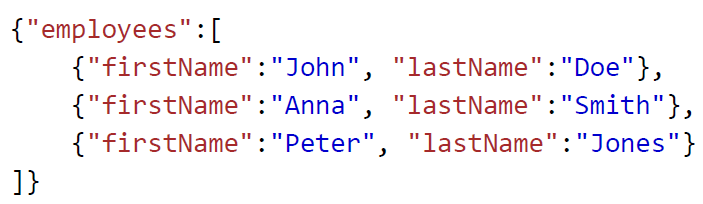
\includegraphics[width=.8\textwidth]{figures/jsonejemplo}
            \end{center}
            \caption{Ejemplo de lista de empleados genérica en \textit{JSON}}
            \label{json-ejemplo}
        \end{figure}
        
        Fue elegido por su compatibilidad con Java y porque es independiente de la tecnología usada en la vista, lo cual permite a su vez realizar cambios en la vista sin afectar las funcionalidades del controlador.
        
        \subsection{JPA}
        \label{tecno-jpa}
        
        Por ``Java Persistence API", proporciona un modelo de persistencia basado en objetos de Java planos (POJO, por sus siglas en inglés \textit{Plain Old Java Object}) para hacer la correspondencia con las entidades en la base de datos\cite{JPA-definicion}. En la práctica, hace transparentes las consultas y acciones realizadas sobre la base de datos.
        
        Como tal, JPA, no implementa los modelos de persistencia que usará la base de datos si no que proporciona un estándar para que se puedan mantener las caractarísticas de la orientación a objetos de Java y se puedan enlazar, uno a uno, con las entidades, atributos y relaciones de la base de datos.
        
        JPA se puede configurar vía anotaciones o usando un documento XML que debe ser distribuido junto con el sistema. En el caso de ``HxPlus Ocupacional" se eligió la configuración por anotaciones debido que está presente directamente en los objetos (clases) de Java y permite una mejor mantinibilidad del código.
        
        Entre las implementaciones conocidas de JPA tenemos:
        \begin{itemize}
             \item Hibernate
             \item ObjectDB
             \item EclipseLink
             \item OpenJPA
        \end{itemize}
        
        Siendo la implementación de Hibernate la seleccionada por lo descrito en el punto \ref{tecno-hibernate}.
        
        \subsection{Angular JS}
        \label{tecno-angular}
        
        Es un \textit{framework}orientada a facilitar el desarrollo web de aplicaciones dinámicas del lado del cilente. ``AngularJS le permite extender el vocabulario HTML para su aplicación"\cite{ANGULARJS-angularjs}. Utiliza lo que llama ``directivas" que son bloques de código en javascript que ayudan a estructurar las acciones del \textit{front-end}. También maneja ``atributos" y ``elementos" que pueden ser programados separadamente del código HTML y luego insertados en dicho archivo para su utilización.
        
        Provee asociación birireccional de variables del DOM lo cual simplifica drásticamente las pruebas del lado del cliente y mantiene, como se mencionó anteriormente, la estructura organizada del código. La asociación bidireccional a través de ``expresiones" se utiliza para mantener actualizado al cliente en cuanto a cambios que se realizen en las variables internas y mejora la respuesta visual sin realizar una recarga de la página.
        
        El código de Javascript (punto \ref{tecno-javascript}) debe ser importado en el archivo HTML en que se quieren utilizar. Existen dos formas de importarlas, desde el servidor de google\footnote{http://ajax.googleapis.com/ajax/libs/angularjs/1.4.8/angular.min.js} o descargando los archivos al servidor local y agregando la dirección local.
        
        Por todo esto, se eligió AngularJS para su utilización como \textit{framework} del \textit{front end} del sistema.
        
        \subsection{JavaScript}
        \label{tecno-javascript}
        
        JavaScript es un lenguaje de programación interpretado, dialecto del estándar ECMAScript. Se define como orientado a objetos, basado en prototipos, imperativo, débilmente tipado y dinámico\cites{JAVASCRIPT-wiki}{JAVASCRIPT-manual}. También posee soporte en casi todos los navegadores utilizados actualmente.
        
        Es un lenguaje de programación orientado a crear contenidos dinámicos para páginas web del lado del cliente. AngularJS, previamente mencionado, usa JavaScript como lenguaje de programación para su implementación.
        
        \subsection{MySQL}
        \label{tecno-mysql}
        
        Manejador de bases de datos, posee licencia GPL y licencia comercial de Oracle\cite{MYSQL-referencemanual}. Ofrece alto rendimiento, eficiencia y seguridad en el almacenamiento y recuperación de datos\cite{MYSQL-oracle}. Comúnmente utilizado en entornos de desarrollo LAMP para desarrollo web.
        
        Es un manejador multi-hilo, multi-usuario y robusto, está diseñado para soportar altos niveles de carga y ser utilizado en entornos de producción con fuerte afluencia de datos. Además de poseer librerías ampliamente usadas para Java las cuales ayudan al desarrollo debilmente acoplado del \textit{back-end}.
        
        Para ``HxPlus Ocupacional" se eliegió este manejador, haciendo uso de su licencia GPL, para el desarrollo del sistema.
        
        \subsection{SPRING}
        \label{tecno-spring}
        
        Framework para el desarrollo de aplicaciones que provee inversión de control; es de código abierto y está diseñado sobre Java. Permite integración con Hibernate, JPA y JSON\cite{SPRING-essential}.
        
        SPRING fue diseñado para facilitar el desacoplamiento de los compomentes del sistema utilizanco IOC. Esto permite que los componentes sean desarrollados una y sólo una vez y que puedan ser reutilizados en diferentes contextos\cite{SPRING-referencedoc}.
        
        Su fácil integración con Hibernate y, por consecuencia, con JPA permite que la interacción con la base de datos sea transparente al desarrollador y evita que tenga que reescribirse el código en caso de cambios en el manejador (de bases de datos) utilizados.
        
        
        \subsection{Maven}
        \label{tecno-maven}
        
        Es una herramienta de gestión y manejo de librerías, parecida a ``Apache Ant". Utiliza el concepto del ``Modelo del Objeto de Proyecto" (del inglés \textit{Project Object Model}, o POM) para gestiónar la construcción del proyecto dónde se utilice. Esto es, gestiona las librerías, dependencias y versiones (de las librerías) de forma centralizada y limpia.
        
        El POM es un archivo en formato XML dónde se registran las librerías que serán usadas por el proyecto  para que el manejador de Maven se encargue de la descarga de las mismas. Se gestiona a través de artefactos que registran la información de una librería de acuerdo con la figura \ref{pom-artifact}.
        
        \begin{figure}[htbp!]
            \begin{center}
                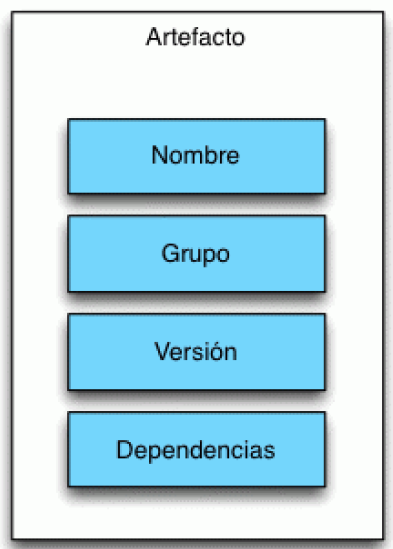
\includegraphics[scale=0.4]{figures/pomartifact}
            \end{center}
            \caption{Artefacto de Maven y descripción de su contenido.}
            \label{pom-artifact}
        \end{figure}
        
        La estructura del POM puede llegar a ser tan compleja como el proyecto que gestiona, llegando incluso a depender de otros POM. En ``HxPlus Ocupacional" se manejó usando un sólo POM de la manera más sencilla posible.
        
        En \citetitle{APACHE-maven}\cite{APACHE-maven} mantienen repositorios de librerías actualizados y correctamente asociados a las dependencias de dichas librerías.
        
        \subsection{Hibernate}
        \label{tecno-hibernate}
        
        Es un framework de persistencia que provee una implementación de JPA\cite{HIBERNATE-basico}. Gestiona las comunicaciones a nivel de nombres de entidades y atributos con su respectiva contraparte de Java, clases con sus atributos. A esto se le conoce como ``Correlación Objeto-Relacional" (ORM, por su siglas en inglés \textit{Object Relational Mapping}).
        
        Esta correlación que crea Hibernate permite ciertas facilidades al momento de manejar las distintas interacciones con la base de datos que devienen en un código mantenible en el tiempo.
        
        El framework es integrado al desarrollo a través de Maven y tiene soporte para los siguientes manejadores de bases de datos\cite{HIBERNATE-tutorial}: 
        \begin{itemize}
            \item MySQL
            \item PostgreSQL
            \item Oracle
            \item DB2/NT
            \item HSQL Database Engine
            \item entre otros...
        \end{itemize}
        
        Tradicionalmente se utilizan dos archivos de configuración (llamados ``hibernate.properties" y ``hibernate.cgf.xml") que se modifican con cada nueva tabla o ``clase de persistencia" que se requiera, sin embargo este método tiende a no ser mantenible en el tiempo ya que debe buscarse dentro de estos archivos las configuraciones de las clases y no existe un orden estipulado para la creación y modificación de estos archivos. Para evitar esto, y dado que se tiene una versión de Java opsterior a JDK 5, se procedió a la utilización de la versión 3 de hibernate que incorpora librerías para el uso de anotaciones, quedando así la configuración de las clases de persistencia dentro del código de las clases de Java, lo cual permite y permitió, durante el desarrollo, fácil depuración de errores y un sencillo mantenimiento del código.
        
        \subsection{iText}
        \label{tecno-itext}
        
        Herramienta de generación de PDF dinámicos\cite{ITEXT-basico}. Proporciona un API que permite la generación de archivos PDF usando la información enviada.
        
        Actualmente existen módulos de gestión, interpretación y conversión de archivos PDF, sin embargo para efectos de ``HxPlus Ocupacional" sólo se utilizó el módulo de generación de los mismos.
        
        Su integración con Maven permitió la fácil descarga de la librería y su configuración dentro del proyecto. Para su uso sólo se necesitó la creación de una clase dentro del \textit{back end}, que contiene las importaciones requeridas para así poder generar los PDF necesarios.
        
    \section{Herramientas para el control de versiones y planificación}
    
    En la presente sección se presentan las herramientas de planificación y control de versiones usadas durante el desarrollo de la aplicación. Si bien no están vinculadas directamente al código, las mismas sirvieron de soporte para la organización del proyecto.
    
        \subsection{Git}
        \label{tecno-git}
        
        Es un sistema de control de versiones distribuido, diseñado por Linus Torvalds, enfocado en eficiencia, integridad de datos, velocidad de transferencia y soporte para flujos de trabajo no lineales.
        
        Siguiendo este enfoque, se logró un \textit{software} que almacena los archivos relativos a un proyecto tomando como base un directorio ``raiz" y los archivos y directorios que lo conformen, incluye recursivamente los archivos y directorios dentro del directorio raiz, y  a partir de ellos almacena los cambios realizados a la última versión, sin modificar los archivos originales ni los archivos de modificaciones; con ello se logra que los cambios puedan ser reversibles y que sean almacenados con poco uso de memoria, reduce la carga de datos al momento de crear repositorios remotos ya que no se está enviando los archivos completos sino los archivos de cambios.
        
        Para el caso de repositorios remotos y el manejo de la carga, también incluye la restricción de versiones. Un usuario debe tener en el repositorio local la última versión disponible, en caso de que la última versión esté en el repositorio local, se cargan los cambios normalmente al repositorio remoto; en caso contrario, el usuario debe descargar la última versión del repositorio remoto, (potencialmente) resolver conflictos que puedan surgir entre los archivos modificados de manera local y los que hayan sido modificados en el servidor remoto y luego hacer la carga al servidor remoto.
        
        También ofrece la posibilidad de crear ``ramas" de desarrollo. Esto es, cambios y modificaciones de un proyecto que parten de una raiz pero que puede tener una meta diferente. Esto facilita el proceso cuando existen varios desarrolladores trabajando en paralelo sobre el mismo proyecto, aunque en el caso de surgir conflictos en los cambios puede llegar a ser engorrosa la integración (\textit{merge}) del código.
        
        Para HxPlus se crearon dos repositorios raices, dadas implicaciones de permisos de ejecución dentro del sistema operativo elegido. Estos repositorios fueron llamasdos ``occupational" y ``proyectoAngular" refiriendose al \textit{back-end} y \textit{front-end} respectivamente.
        
        \subsection{GitHub}
        \label{tecno-github}
        
        Servidores online de repositorios remotos para Git. Puede ser usado de manera gratuita y pública. Permite el acceso a los repositorios de manera ininterrumpida y global.
        
        Los repositorios fueron almacenados en la cuenta personal de Alejandro Tarazona, en el url: \textit{http://www.github.com/atarazona89} con los nombres descritos con anterioridad, para su almacenamiento en la web.
        
        \subsection{Trello}
        \label{tecno-trello}
        
        Herramienta diseñada con la misión de facilitar la gestión de tareas usando listas o tablas. Cuenta con una interfaz intuitiva y de fácil aprendizaje para llevar a cabo dicha misión. Una vez creadas las tablas que se desean, se pueden crear tareas dentro de ellas, las cuales a su vez pueden ser etiquetadas, organizadas o comentadas por los participantes. Las tareas pueden ser arrastradas entre las listas emulando así la transición entre los estados de desarrollo del proyecto.
    
\pagebreak
     \chapter{Desarrollo de la Aplicación}
\label{desarrollo-capitulo}
%En el presente capítulo se presenta, de forma detallada, cómo fue el desarrollo del proyecto y finaliza con una revisión de dificultades técnicas y los resultados del proyecto.

El presente capítulo describe las etapas del desarrollo de la aplicación. Además se presentan las dificultades técnicas encontradas a lo largo del mismo y el resultado final alcanzado.

El desarrollo se dividió en tres fases:

\begin{enumerate}
    \item Fase de Inicio.    
    \item Fase de Implementación.
    \item Fase de Cierre.
\end{enumerate}

Previo a la realización de estas fases, se llevó a cabo una fase para la descarga e incialización de las herramientas a ser utilizadas en el desarrollo de la aplicación. Además se crearon las cuentas para el manejo de  los repositorios del proyecto

Cada fase posee sus propios objetivos generales y específicos, la fase de implementación contempla también los \textit{Sprint} realizados siguiendo la metodología seleccionada.

\section{Fase de Inicio}
    
    \textbf{\underline{Objetivo General:}}
    Llevar a cabo el levantamiento de requerimientos e identificación de los módulos a desarrollar en el proyecto.
    
    \textbf{\underline{Objetivos Específicos:}}
    \begin{itemize}
        \item Levantamiento de los requerimientos del sistema.
        \item Identificación de los módulos que conformarán el sistema a desarrollar.
        %\item Descarga y configuración de Eclipse, JSON, Hibernate, Liquibase, Maven, AngularJS, Apache y Tomcat.
        %\item Creación de cuentas para el manejo de los repositorios del proyecto y \textit{Product Backlog}.
        \item Creación del \textit{Product Backlog}.
        \item Elaboración del diagrama inicial de base de datos. %y casos de uso.
        \item Evaluación de restricciones y riesgos por parte del equipo de desarrollo.
    \end{itemize}
    
    En esta fase se realizó, en conjunto con el ing. Juán Albarrán, el levantamiento de los requerimientos funcionales y no funcionales del sistema, dichos requerimientos fueron:
    
    \subsection{Requerimientos Generales}
    \begin{itemize}
        \item El sistema debe poseer mecanismos de autenticación para la verificación de identidad.
        
        \item El sistema debe proveer una plataforma de almacenamiento de historiales médicos con asociaciones entre la empresa en la que trabaja el paciente, la sucursal o ``centro de costos"\footnote{Se usa el término \textit{Centro de Costos} para referirse a una sucursal o sede donde haya personal tabajando.} en el cual trabaja el paciente al momento de la consulta.
        
        \item Mantener los historiales a través del tiempo, sin importar los cambios de ``centro de costos", que presente el paciente, ni el médico que lo atienda.
        
        \item En casos de algún cambio en el centro de costos donde trabaja el paciente, se deberán especificar como terminación o renovación de contratos de parte de los usuarios y la empresa.

    \end{itemize}        
        
        Todo esto con la finalidad de poder realizar cruces de información e investigación de causas de enfermedades tomando en cuenta los lugares de trabajo y las tareas desempeñadas por los trabajadores.
        
    \subsection{Requerimientos Específicos}
    
    \begin{itemize}
        \item \textbf{\underline{Usuarios:}}
        
        Fue modelado como ``Usuario" todo aquel empleado de una empresa registrada en el sistema. Para efectos del presente proyecto, los usuarios son los trabajadores de las empresas. Se hace una diferencia especial a dos tipos específicos de usuario: el doctor y el paciente (no excluyentes) que son la línea principal de trabajo del sistema. El sistema debe ser capaz de mantener una base de datos de usuarios con los atributos especificados en el Apédice \ref{ere}.
        
        La categoría de ``Doctor" en una empresa se refiere al personal médico calificado para realizar consultas y diagnósticos médicos, por consecuencia será representado como un contrato especial y, sin discriminación por la especialidad o nivel de instrucción del mismo, será almacenado en el sistema con el nombre de ``Doctor". En la sección de almacenamiento de los datos del doctor, será  almacenada la información específica del mismo.
        
        Los ``Pacientes" por otro lado representan a todo el personal que haya sido atendido y tenga su historia médica registrada en el sistema. Cabe destacar que un ``Doctor" puede también ser paciente, aunque no puede ser su propio paciente.
        
        \item \textbf{\underline{Historial Médico:}}
        
        El historial médico de un paciente se realiza al momento de la primera consulta que sea registrada en el sistema, en ese momento de registran:
        
        \begin{enumerate}
            \item Antecedentes o Trasfondos: Enfermedades diagnosticadas previamente al paciente así como predisposiciones a enfermedades hereditarias.
            \item Hábitos: Son actividades regulares del paciente. Pueden variar en tipo y frecuencia. Éstos pueden ser habitos recomendados o perniciosos para el paciente. La finalidad es que las investigaciones de enfermedades ocupacionales puedan descartar los hábitos de los pacientes como factores.
            \item Alergias: También se registran alergias diagnosticadas al paciente. Se realiza en una sección a parte de los trasfondos debido a que las alergias poseen características específicas y se manifiestan sólo con la presencia del alérgeno\footnote{Según el diccionario de la RAE: \textit{alérgeno, na}: 1. adj. Perteneciente o relativo a los alérgenos. 2. m. Sustancia antigénica que induce una reacción alérgica en un organismo.} correspondiente.
            \item Vacunas: Por último ser registran las vacunas que posee el paciente detallando el nombre y la potencia en caso en que aplique (vacunas de varias dosis o refuerzos).
        \end{enumerate}
        
        El usuario debe estar previamente registrado y contratado por la empresa que contrata al doctor para poder crearse su historial médico.
        
        \item \textbf{\underline{Consultas Médicas:}}
        \label{consultas-datos}
        
        Una vez creado el historial médico pueden realizarse consultas médicas. En ellas se registrará la información recogida durante dicha consulta y se almacenará en el sistema.
        
        Basándose en la información recopilada por Globinsoft S.A. para su proyecto ``HxPlus" (principal antecedente del presente proyecto), queda establecida la estructura de una consulta de la siguiente forma:
        
        \begin{enumerate}
            \item \textit{SoapNote} (nota de revisión): Usada por los médicos para organizar las consultas y que consta de:
            \begin{enumerate}
                \item Subjective: Información subjetiva, comunmente redactada en lenguaje informal, que contiene lo que el paciente describe, dolencias y síntomas presentados.
                \item Objective: Información objetiva recopilada por el médico durante la consulta. Redactada en lenguaje formal.
                \item Assessment: Comentarios u observaciones realizados por el médico.
                \item Plan: Plan acción a realizar para tratar las dolencias.
            \end{enumerate}
            \item Diagnóstico(s): Uno o varios diagnósticos realizados por el médico en la consulta.
            \item Instrucción(es): Una o varias instrucciones. Acciones que deben ser llevadas al pie de la letra en cuanto a conductas o hábitos del paciente, se incluye en este apartado regulaciones alimenticias y recomendaciones periódicas.
            \item Prescripción(es): Instrucciones de uso de medicamentos registrados en el sistema junto con la información de dicho medicamento. Con esto se podrán generar los récipes médicos para la adquisición de fármacos que así lo requieran.
            \item Signos Vitales: Se registran los signos vitales recabados en la consulta. Dado que puede variar los signos vitales pertinentes entre las distintas especialidades de la medicina, se deja a juicio del médico tratante qué signos vitales serán tomados en la consulta.
            \item Solicitud y Recepción de exámenes médicos: En la primera se registra una solicitud de un examen dado. En una futura consulta puede darse por recibido en el sistema el examen médico y adjuntar el archivo respectivo para su almacenamiento. Se puede solicitar o recibir más de un examen médico por consulta.
        \end{enumerate}
        
        El sistema debe ser capaz de almacenar y desplegar esta información ordenada cronológicamente a partir de la consulta médica más reciente.
        
        \item \textbf{\underline{Reportes Médicos:}}
        
        El sistema debe poder generar de manera automática los reportes médicos con la información recopilada en las consultas a solicitud del médico.
    \end{itemize}
    
    Todos estos requerimientos fueron archivados en notas para la realización del \textit{Product Backlog} utilizando el sistema Trello y se enlazó con la pizarra creada por el \textit{Scrum Manager} para la gestión del proyecto.
    
    Se dividió el proyecto en ``módulos" y éstos a su vez en ``vistas" las cuales pasaron a ser la unidad granular deseada para el manejo del proyecto, quedando así la primera versión de la lista del producto de la siguiente forma:
    
    \begin{enumerate}
        \item \textbf{\underline{Módulo de Autenticación:}}
        
        \begin{itemize}
            \item Vista de autenticación: Incluye inicio y cierre de sesión dentro del sistema.
        \end{itemize}
        
        \item \textbf{\underline{Módulo de Gestión de Usuarios:}}
        
        \begin{itemize}
            %\item Vista de Agregar Usuario: Formulario de creación de usuarios nuevos en el sistema.
            \item Vista de Lista de Usuarios: Lista de los usuarios registrados en el sistema. Esta vista será refinada en el futuro para que haga discriminación entre usuarios por empresa (ej. un usuario de una empresa A no podrá ver la lista de otra empresa B ni éstos aparecerán en su lista).
            \item Vista de Detalles de Usuario: Vista de los datos personales de un usuario.
            \item Vista de Edición de Usuario: Formulario lleno con los datos personales de un usuario.
        \end{itemize}
        
%        \item \textbf{\underline{Módulo de Doctores:}}
%        \begin{itemize}
%            \item Vista de Agregar Doctor: Formulario para el registro de un nuevo dorctor en la empresa.
%            \item Vista de Lista de Doctores: Lista con los doctores contratados por una empresa.
%            \item Vista de Detalles de Doctor: Vista de los datos característicos de un doctor.
%            \item Vista de Edición de Doctor: Formulario lleno con los datos profesionales de un doctor dado. Se usa para la actualización de dichos datos.
%        \end{itemize}
        
        \item \textbf{\underline{Módulo de Pacientes:}}
        \begin{itemize}
            \item Vista de Añadir Nuevo Paciente: Al añadir un nuevo paciente, el doctor puede añadir un nuevo paciente a su lista de pacientes atendidos y el mismo puede provenir de las listas de usuarios atendidos previamente y que estén contratados por la empresa o ser un paciente totalmente nuevo, en tal caso pasaría a la siguiente vista.
            \item Vista de Lista de Pacientes Atendidos: El doctor tiene a su disposición una lista de pacientes que ha atendido con anterioridad, ordenada por fecha de última consulta médica y se mostrarán los pacientes atendidos más recientemente primero.
            \item Vista de Creación de Historia Médica: Formulario con el cual se añaden los datos necesarios para la creación de una nueva historia médica al sistema. Usado en el caso de que un paciente esté siendo atendido por primera vez desde su registro en el sistema (no importa si ha cambiado de puesto de trabajo, sólo se discrimina por el puesto actual).
        \end{itemize}
        
        \item \textbf{\underline{Módulo de Consultas Médicas:}}
        \begin{itemize}
            \item Vista de Historial de Consultas Médicas del Paciente: Una lista de las consultas que ha tenido el paciente ordenadas cronológicamente empezando desde la última consulta.
            \item Vista de Agregar Consulta Médica: Formulario con los datos requeridos para almacenar una consulta médica nueva.
            \item Vista de Revisión de Consulta Médica: En esta vista se despliegan los datos almacenados de una consulta médica ya realizada. También se accede a los archivos previamente almacenados (exámenes médicos recibidos) y a la funcionalidad de generación de reportes.
            \item Vista de Generación de Reportes Médicos: En esta vista de podrán elegir los reportes que serán generados por el sistema.            
        \end{itemize}
    \end{enumerate}
    
    Todo esto quedó plasmado en el sistema de pizarras de Trello asociado a la cuenta del equipo de desarrollo.
    
    Basándose en los requerimientos recopilados, el equipo de desarrollo, realizó un diagrama de base de datos el cual a su vez fue modificado durante el desarrollo del proyecto. La versión final del mismo puede ser consultado en el Apéndice \ref{ere}.
    
    Del análisis de riesgos del proyecto, se obtuvo la siguiente lista de riesgos:
    
    \begin{enumerate}
        \item \textbf{Equipo de desarrollo pequeño:} Dado que se cuenta con un sólo integrante del equipo de desarrollo los avances en la implementación del proyecto deben ser pequeños con la intención de que sean funcionales y estén probados.
        \item \textbf{Falta de diversidad en el conocimiento:} También por ser un grupo pequeño, pueden surgir, durante el desarrollo, impedimentos por falta de dominio de las herramientas. En tal caso se deberá realizar una fase de capacitación para las fases impedidas lo cual podría retrasar las entregas.
        \item \textbf{Tiempo dedicado a los \textit{Sprint}:} Si los \textit{Sprint} son establecidos en una o dos semanas, los avances podrán verse rápidamente, aunque serían poco avance. Por otro lado, mantener el tiempo de \textit{Sprint} en tres o cuatro semanas, se verían pocos avances y la retroalimentación sería escasa. Para solventar tal riesgo, se designó un tiempo de \textit{Sprint} variable, quedando establecido un tiempo de dos semanas para aquellas vistas en las que el equipo de desarrollo no precise capacitación y de tres a cuatro semanas para las que si sea necesaria la capacitación.
    \end{enumerate}
    
    En paralelo a la realización de este trabajo, se realizó la descarga Eclipse Kepler, descargado desde la página oficial de Eclipse\cite{ECLIPSE-eclipseorg}, Apache, Tomcat (ambos descargados de \cites{APACHE-maven}{APACHE-tomcat} respectivamente) y las librerías de AngularJS.
    
    Se procedió a la configuración de Maven y se agregaron las dependencias iniciales para usar \textit{SPRING} como \textit{framework}, Hibernate y Liquibase como gestores de comunicación con la base de datos y configurar la base de datos con las credenciales de MySQL asignadas para el desarrollo del proyecto.
    
    \begin{table}[h!]
        
        \begin{center}
            \begin{tabular}{|l|l|l|}\hline
                Grupo & Artefacto & Versión \\\hline
                org.springframework & spring-core & 4.1.2.RELEASE \\\hline
                org.springframework & spring-orm & 4.1.2.RELEASE \\\hline
                org.springframework & spring-webmvc & 4.1.2.RELEASE \\\hline
                mysql & mysql-connector-java & 5.1.9 \\\hline
                org.liquibase & liquibase-plugin & 1.6.1.0 \\\hline
            \end{tabular}
        \end{center}
        
        \caption{Artefactos de Maven: Spring}
        \label{artefactos-spring}
    \end{table}
    
    Aunque, en lo referente a liquibase, se utilizó un plugin, no una librería. Ver tabla \ref{artefactos-spring}.
    
    Se realizaron los cambios dentro del archivo ``occupational-servlet.xml" que permite el uso de anotaciones para el direccionamiento interno de los procesos.
    
    Usando los repositorios de Maven se descargaron las librerías necesarias de JSON para la comunicación. Las dependencias descargadas fueron del grupo \textit{com.fasterxml.jackson.core}, las enumeradas en el tabla \ref{artefactos-json}.
     
    \begin{table}[h!]
         
        \begin{center}
            \begin{tabular}{|l|l|}\hline
                Artefacto & Versión \\\hline
                jackson-core & 2.2.2 \\\hline
                jackson-annotations & 2.2.2 \\\hline
                jackson-databind & 2.2.2 \\\hline                   
            \end{tabular}
        \end{center}
        
        \caption{Artefactos de Maven: JSON}
        \label{artefactos-json}
    \end{table}
    
    También, usando Maven, fueron descargadas las librerías de Hibernate que usan JPA como API para comunicarse con la base de datos (tabla \ref{artefactos-hibernate}).
    
    \begin{table}[h!]
        
        \begin{center}
            \begin{tabular}{|l|l|l|}\hline
                Grupo & Artefacto & Versión \\\hline
                org.hibernate.javax.persistence & hibernate-jpa-2.0-api & 1.0.1.Final \\\hline
                org.hibernate.common & hibernate-commons-annotations & 4.0.4.Final \\\hline
                javax.persistence & persistence-api & 1.0.2 \\\hline
                org.hibernate & hibernate-entitymanager & 4.1.9.Final \\\hline
                org.springframework.data & spring-data-jpa & 1.8.1.RELEASE \\\hline
            \end{tabular}
        \end{center}
        
        \caption{Artefactos de Maven: Hibernate}
        \label{artefactos-hibernate}
    \end{table}
    
\section{Fase de Implementación} 

En esta fase se realizó en sí el desarrollo del sistema. Hubo modificaciones en el diagrama de base de datos (versión final en Apédice \ref{ere-diagrama}) y, los requerimientos que cambiaron, se reflejaron en el \textit{product backlog} conforme fueron sucediendo.

La implementación se subdividió en Sprints y, como se menciona anteriormente, estos fueron de duración variable.

Cabe destacar que dado que los módulos referentes al manejo de empresas (``Compañía", ``Agregar Usuario", ``Contratos" y la gestión de doctores) están por fuera del alcance del proyecto, se utilizó una base de datos de pruebas generada exclusivamente para tal fin. También fueron generados datos de prueba para medicamentos y laboratorios, por las mismas razones expresadas con anterioridad.

    \subsection{Primer Sprint: Vista de Autenticación de Usuarios}
    Se implementó la funcionalidad de autenticación siguiedo los parámetros de autenticación basada en \textit{tokens}, para ello se agregó al ``pom.xml"\footnote{Ver punto \ref{tecno-maven}} las dependencias requeridas para la autenticación. Ver tabla \ref{artefactos-tba}
    La clave usada por el servidor fue una clave generada en tiempo de ejecución para que la misma fuera cambiante y mejorar la seguridad. Sin embargo, la clave, una vez generada se mantiene igual mientras el servidor esté en funcionamiento. Ver figura \ref{Autenticación}.
    
    \begin{figure}[htbp!]
        \begin{center}
            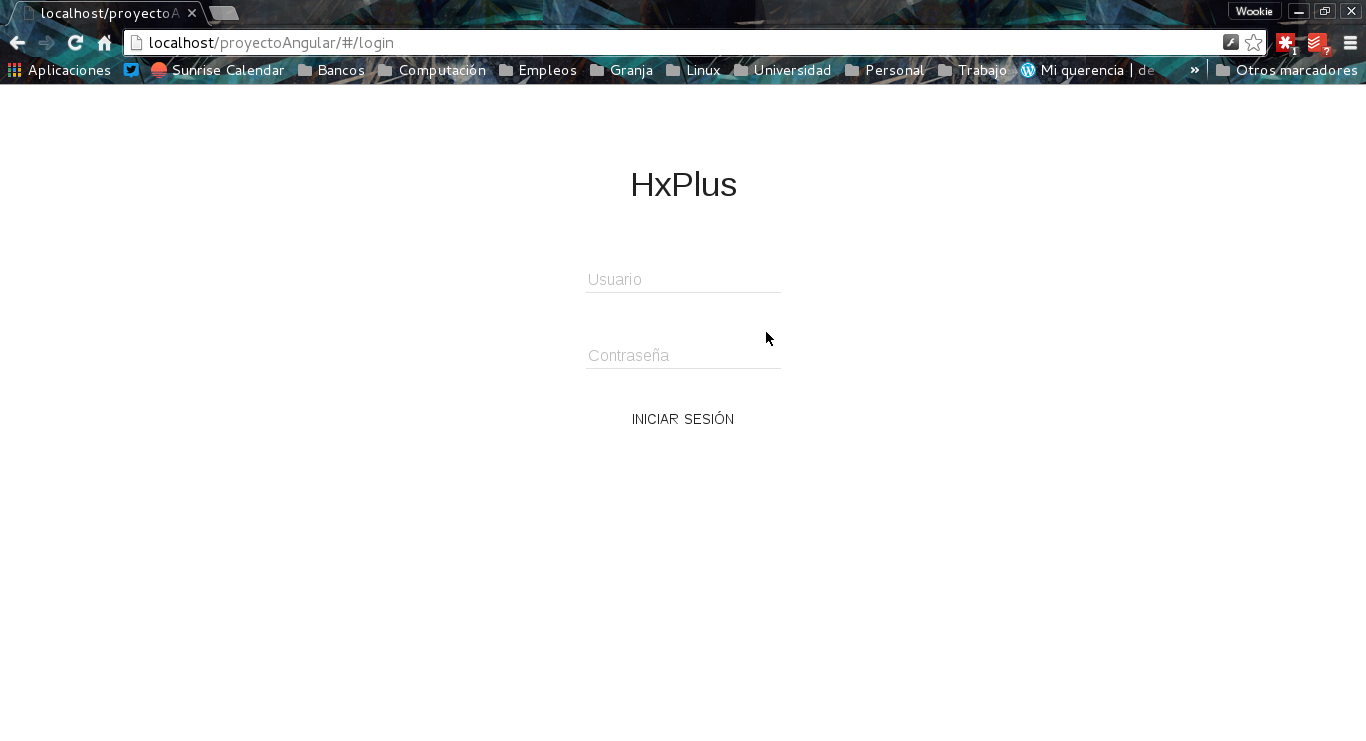
\includegraphics[width=.9\textwidth]{figures/p1}
        \end{center}
        \caption{Pantalla de Autenticación de usuarios}
        \label{Autenticación}
    \end{figure}
    
    \begin{table}[h!]
        
        \begin{center}
            \begin{tabular}{|l|l|l|}\hline
                Grupo & Artefacto & Versión \\\hline
                io.jsonwebtoken & jjwt & 0.5.1 \\\hline
            \end{tabular}
        \end{center}
        
        \caption{Artefactos de Maven: Autenticación}
        \label{artefactos-tba}
    \end{table}
    
    Las pruebas sobre esta vista fueron realizadas evaluando la generación del \textit{token} de parte del servidor en \textit{back end} y su posterior uso para el acceso a las demás páginas del sistema. La ficha fue generada con éxito y verificado el cambio de ficha en cada inicio de sesión, se dió la aprobación de la vista para proseguir al siguiente Sprint.
    
%    \subsection{Segundo Sprint: Vista de Agregar Usuario}
%    
%    En esta vista se buscó crear un formulario con los datos de un usuario nuevo que serán agregados al sistema. Los datos para el mismo fueron:
    
%    \begin{itemize}
%        \item Nombre de usuario: El apodo que tendrá el usuario en el sistema.
%        \item Contraseña: La contraseña que será utilizada para verificar la identidad del usuario. Se reqiuere que sea introducida dos veces al sistema para evitar errores posteriores.
%        \item Cédula de Identidad: El número de cédula es el documento de identificación del usuario en el país.
%        \item RIF: Registro de información fiscal. También es un método de identificación del usuario en el país.
%        \item Nombre: Indica el primer nombre del usuario. No se hace mención al segundo nombre dado que no es estrictamente necesario para el sistema y sería una carga extra para la transferencia de datos.
%        \item Apellido: Indica el primer apellido del usuario.
%        \item Sexo.
%        \item Fecha de nacimiento.
%        \item Correo Electrónico: Correo electrónico del usuario al cual contactarle en caso de ser necesario. También es usado para verificar la identidad del usuario y evitar que sea registrado dos veces en el sistema.
%        \item Dirrección: La dirección de habitación del usuario.
%        \item Número de Teléfono: El número de teléfono al que se pueda contactar al usuario.
%    \end{itemize}
    
%    A este Sprint se le asignó un tiempo de dos semanas debido a que, a pesar se la sencillez del mismo, el equipo de desarrollo no poseía los conocimientos técnicos específicos para el manejo de AngularJS y requirió capacitación previa para solventarse. Para ello se utilizó como referencia \cite{CODESCHOOL-main} en su curso ``Shaping up with Angular.js" que hace referencia al manejo de AngularJS desde el diseño de UI hasta manejo de los datos del lado del cliente.
    
%    Las pruebas fueron realizadas usando los siguientes criterios:
    
%    \begin{enumerate}
%        \item Agregar un usuario con un apodo ya existente.
%        \item Agregar un usuario con un número de cédula o RIF ya existentes.
%        \item Agregar un usuario sin alguno de los campos requeridos (nombre de usuario, contraseña, primer nombre, primer apellido, número de cédula y correo electrónico).
%    \end{enumerate}
    
    \subsection{Segundo Sprint: Vista de Lista de Usuarios}
    
    Esta vista contiene una lista con los nombres de los usuarios registrados en el sistema. Para el alcance del sistema se implementó una lista general sin discriminaciones sobre dicha lista y fue utilizada en las pruebas de la vista de ``Detalles de Usuario". Se plantea que a futuro sea utilizada por usuarios especiales dentro del sistema y que manejen dichas listas dentro de una empresa.
    
    A este Sprint se le asignó una semana de lapso para su entrega dada la importancia relativamente baja de la vista no se refinó y su UI está muy poco refinada.
    
    Las pruebas de la vista se basaron en el orden de aparición de los usuarios (ordenados alfabeticamente) y la actualización de la lista al agregar un nuevo usuario.
    
    \subsection{Tercer Sprint: Vista de Detalles de Usuario}
    
    Esta vista es la muestra de los datos ingresados al sistema del usuario elegido.
    
    A este Sprint, debido a su simpleza, se le dedicó sólo una semana de tiempo para realizar las pruebas necesarias.
    
    Por ser una vista sencilla, las pruebas se realizaron correlacionando los datos de los usuarios con lo que se muestra en pantalla y la aceptación de UI por parte del \textit{product owner} (figura \ref{Revisión}).
    
    \begin{figure}[htbp!]
        \begin{center}
            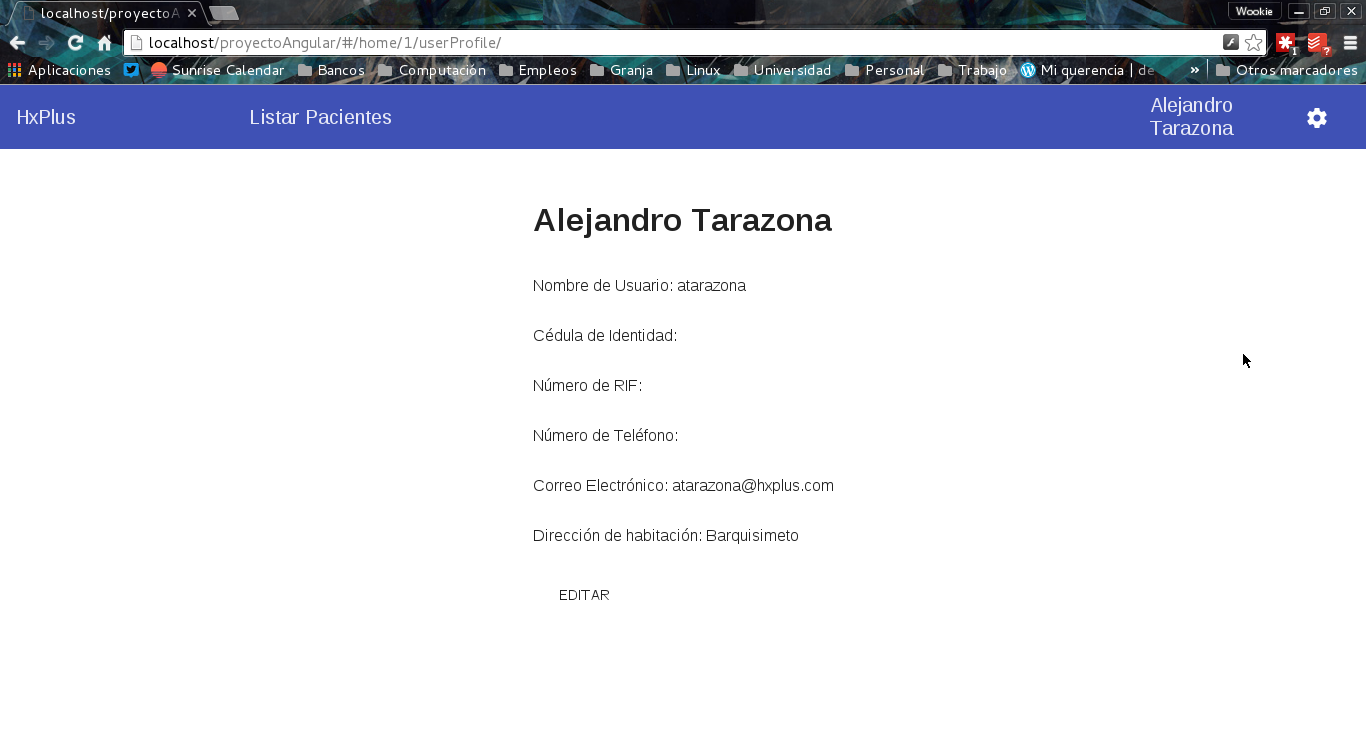
\includegraphics[width=.9\textwidth]{figures/p3}
        \end{center}
        \caption{Pantalla de Detalles de Usuario.}
        \label{Revisión}
    \end{figure}
    
    \subsection{Cuarto Sprint: Vista de Edición de Usuario}
    
    Esta vista muestra un formulario, similar al formulario de registro de usuario, lleno previamente con los datos  previamente registrados. Si el formulario cambia y estos cambios son enviados, el sistema los almacena y regresa a la vista anterior, en caso de éxito, y muestra los datos actualizados del usuario. En caso de algún fallo, el sistema debe dar el mensaje correspondiente al cambio ilegal y mantenerse en la vista con los datos originales del usuario. En caso de modificaciones de la contraseña, el usuario no podrá ver la contraseña previa y el campo estará vacío; este campo se llenará en caso de desear modificarla y se necesita también una verificación de doble escritura de la contraseña para tal fin.
    
    Las pruebas de esta vista fueron:
    \begin{enumerate}
        \item\label{required} Alterar la información del usuario eliminando campos requeridos (nombre de usuario, contraseña, primer nombre, primer apellido, número de cédula y correo electrónico).
%        \item\label{password} Cambiar la contraseña con errores en la doble verificación de escritura.
        \item\label{repeated} Cambiar el nombre de usuario, número de cédula o correo electrónico por valores ya registrados en el sistema.
        \item\label{no-alter} No alterar ningún dato del usuario y enviar el formulario con los datos previos usando el botón de envío de datos.
        \item\label{details} Verificar que los datos fuesen actualizados en la vista anterior en caso de haber verificaciones válidas en el usuario dado.
    \end{enumerate}
    
    A partir del caso \ref{repeated} se detectó que el sistema realizaba una modificación completa del usuario en la base de datos con los datos enviados en el formulario, lo cual podría devenir en problemas de procesamiento a futuro con grandes cargas de datos y es innecesario en el caso \ref{no-alter} por la misma naturaleza de la no modificación. Se acordó, en el siguiente Sprint, revisar esta funcionalidad (figura \ref{Edición}).
    
    \begin{figure}[htbp!]
        \begin{center}
            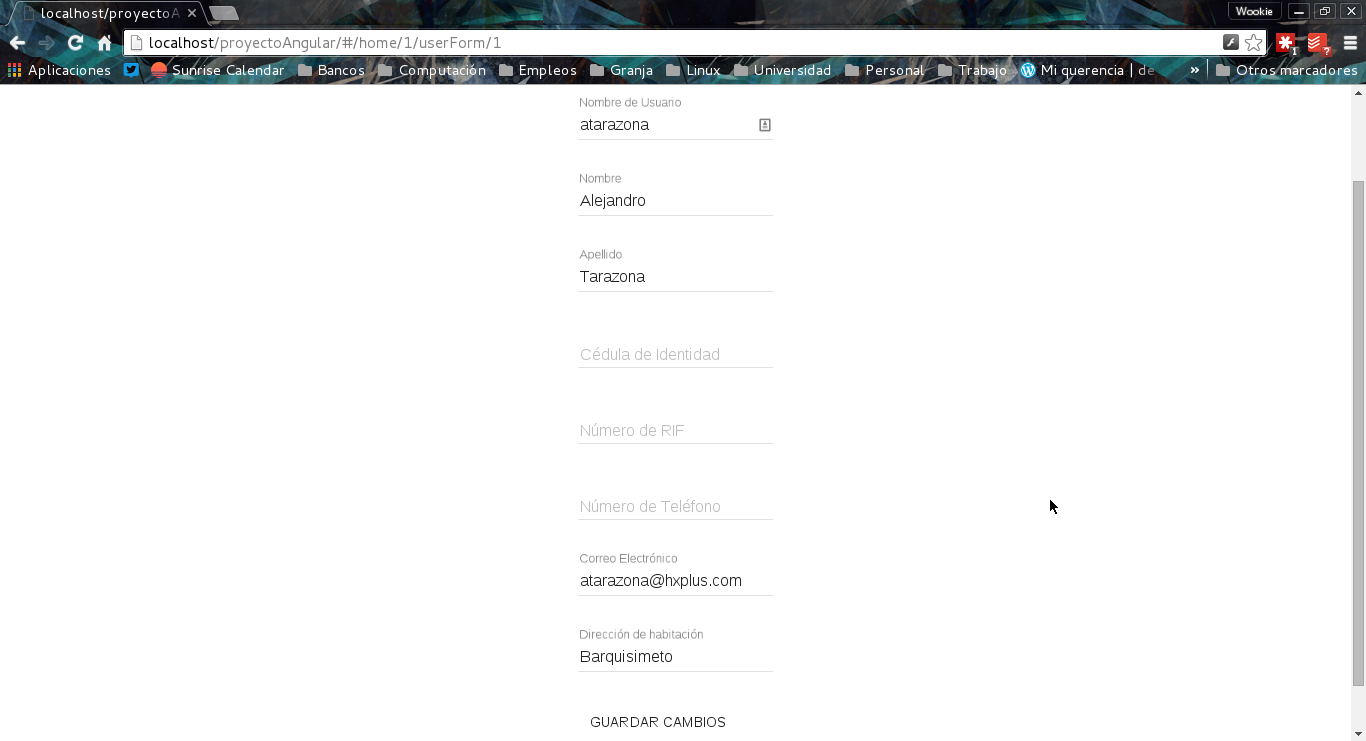
\includegraphics[width=.9\textwidth]{figures/p5}
        \end{center}
        \caption{Pantalla de Edición de Usuario.}
        \label{Edición}
    \end{figure}
    
    A este Sprint, dada la poca complejidad que presenta, se le asignó una semana de duración pero, debido a los errores encontrados en la implementación, se le asignó una semana adicional de revisión adicional dentro del siguiente Sprint.
    
%    \subsection{Quinto Sprint: Vista de Agregar Doctor}%
%    \subsection{Sexto Sprint: Vista de Lista de Doctores}
%    \subsection{Sexto Sprint: Vista de Detalles del Doctor}
%    \subsection{Septimo Sprint: Vista de Edición de Doctor}
    \subsection{Quinto Sprint: Vista de Añadir Nuevo Paciente y Revisón de la Edición de Usuario}
    
    Se realizó la revisión de la ``Vista de Edición de Usuario" debido a que presentaba sobrecarga de datos y en el caso de la no modificación del usuario se reescribían los datos con los mismos valores. El problema fue solventado agregando un detector de cambios con el cual sólo los datos modificados son enviados en el formulario, con esto se logra, no sólo reducir la cantidad de datos enviados al servidor si no que también se elimina la sobrecarga en caso de enviar un formulario con datos idénticos a los que fueron recibidos.
    
    Por otro lado, en la ``Vista de Añadir Nuevo Paciente", el doctor tiene la opción de elegir entre:
    
    \begin{enumerate}
        \item\label{list} Un paciente que ya posea historia médica en el sistema:\\
        Se creó una lista de pacientes cuyos historiales médicos estén registrados en el sistema y serán agregados a la lista de pacientes del doctor (figura \ref{Agregar}).
        \item\label{new} Crear la historia médica de un usuario, ya registrado, que no la posea.\\
        Para este caso se planificó agregar un botón de redirección a la ``Vista de Crear Historia Médica", descrita posteriormente, y que actualizaría la lista de pacientes con historia médica y dejaría en selección el nuevo paciente ya creado.
    \end{enumerate}
    
     Para este Sprint la fase de pruebas de esta vista fue aceptación de la UI y revisión de la acción mencionada en el punto \ref{list} dentro de la base de datos dado que no se cuenta con la vista necesaria y esta será desarrollada en el próximo Sprint.
    
    Se dedicó, en total, dos semanas a este Sprint, dejando para futuros Sprint las pruebas mencionadas.
    
    \begin{figure}[htbp!]
        \begin{center}
            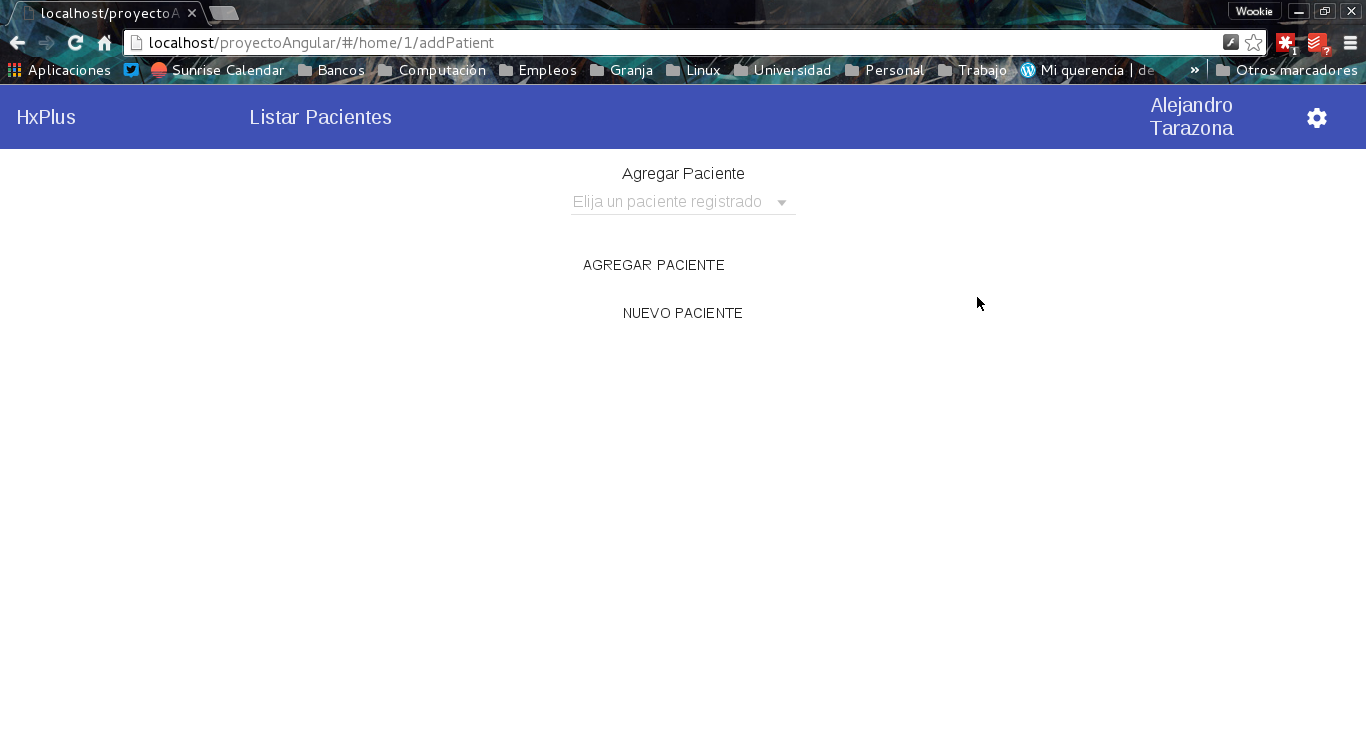
\includegraphics[width=.8\textwidth]{figures/p8}
        \end{center}
        \caption{Vista de Agregar pacientes que ya han sido atendidos por algún médico.}
        \label{Agregar}
    \end{figure}
    
    \subsection{Sexto Sprint: Vista de Lista de Pacientes Atendidos}
    
    En esta vista se presentan por orden alfabético los pacientes que han sido atendidos por el doctor. Además, se presenta la opción de revisar su historial médico con lo cual se desplegará la ``Vista de Historial de Consultas Médicas del Paciente" (ver punto \ref{historial-medico}).
    
    Esta vista se usó como referencia para las pruebas de la ``Vista de Agregar Nuevo Paciente" para revisar que la agregación estaba siendo realizada exitosamente.
    
    Para este Sprint se dedicó una semana y las pruebas se basaron en la respuesta de la vista ante los cambios realizados por la vista mencionada y en la aceptación de la UI (figura \ref{Pacientes}).
    
    \begin{figure}[htbp!]
        \begin{center}
            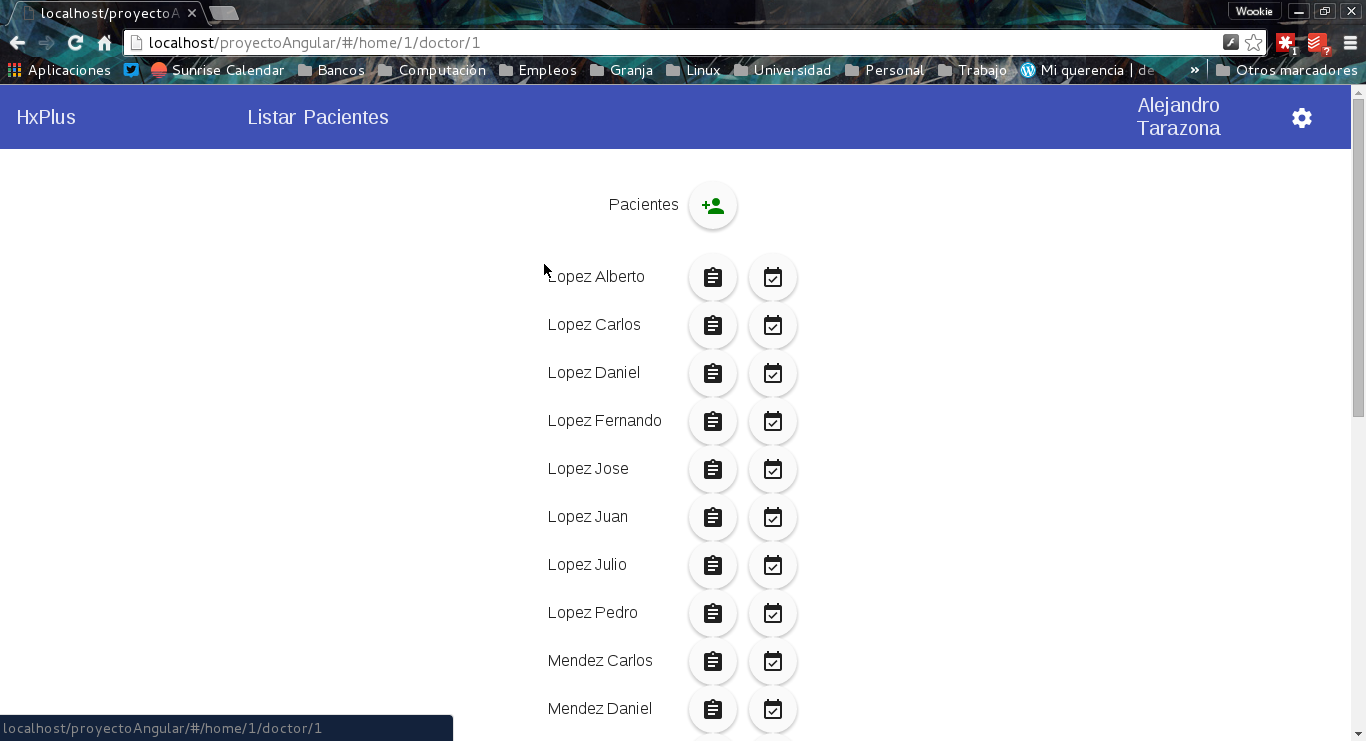
\includegraphics[width=.9\textwidth]{figures/p6}
        \end{center}
        \caption{\label{Pacientes}Lista de Pacientes del Médico}
    \end{figure}
    
    \subsection{Septimo Sprint: Vista de Creación de Historia Médica}
    
    En esta vista se presenta un formulario dinámico\footnote{Flexible en la cantidad de valores que puede aceptar un mismo campo. Puede verse como un ejemplo de un campo multivaluado de un diagrama ER-E} con los campos requeridos para la creación de la historia médica del paciente.
    
    Los campos que admiten más de un sólo valor son:
    \begin{itemize}
        \item Alergias.
            \begin{itemize}
                \item Nombre
                \item Descripción
                \item Severidad
            \end{itemize}
        \item Hábitos.
            \begin{itemize}
                \item Nombre
                \item Frecuencia
            \end{itemize}
        \item Vacunas.
            \begin{itemize}
                \item Nombre
                \item Potencia
            \end{itemize}
    \end{itemize}
    
    Se realizó la subdivisión de acuerdo a los avances realizados por Globinsoft S.A. y están encapsuladas de tal forma que se pueden agregar o eliminar de forma independiente una alergia, un hábito o una vacuna a la lista respectiva sin la necesidad de refrescar o recargar la página. Todos los datos recaudados son enviados una y sólo una vez al servidor una vez seleccionada la opción de envío del formulario.
    
    Las enfermedades diagnosticadas previamente son un único valor dado que puede no ser precisa la información suministrada por el paciente.
    
    \begin{figure}[htbp!]
        \begin{center}
            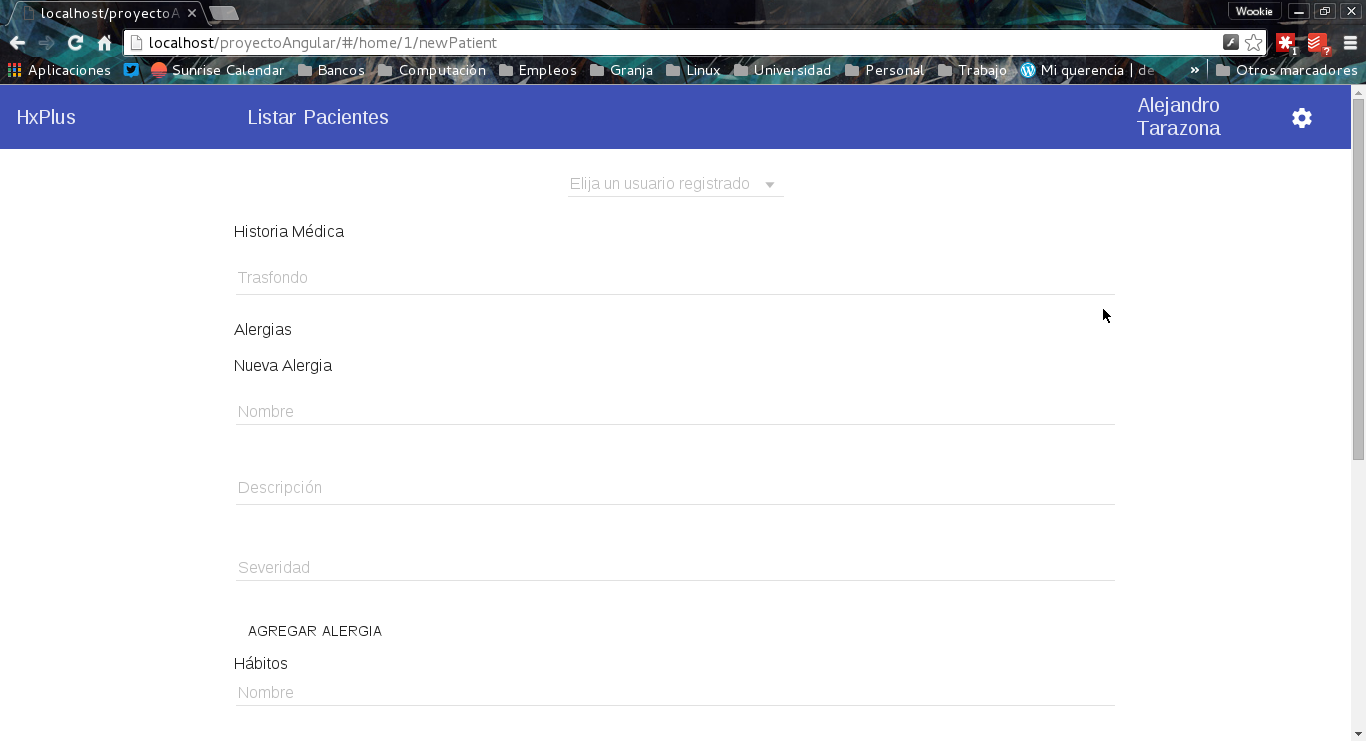
\includegraphics[width=.9\textwidth]{figures/p10}
        \end{center}
        \caption{Vista de creación de nueva historia médica para un paciente nuevo.}
        \label{creación}
    \end{figure}
    
    Debido a la complejidad de la implementación de los formularios dinámicos, se asignaron tres semanas para la implementación exitosa de esta vista (figura \ref{creación}). Las pruebas fueron realizadas basándose en:
    
    \begin{enumerate}
        \item Respuesta a agregación o eliminación de valores en los campos dinámicos.
        \item Carga y comunicación con el servidor.
        \item Revisión de la creación de la historia médica (por verificar luego de la implementación del punto \ref{historial-medico}).
    \end{enumerate}

    \subsection{Octavo Sprint: Vista de Agregar Consulta Médica}
    \label{crear-consulta}
    
    En esta vista se presentan los formularios respectivos para la creación de una nueva consulta médica separados por subvistas que van llenando cada una de los aspectos requeridos de las consultas médicas tal y como se enumeraron en \ref{consultas-datos} y subdivididos en:
    
    \begin{itemize}
        \item Resumen General (figura \ref{img-revisiongeneral}):
            \begin{itemize}
                \item Análisis Subjetivo (\textit{Sujective})
                \item Análisis Objetivo (\textit{Objective})
                \item Plan de tratamiento
                \item Diagnóstico(s)\\
                En este caso se hizo uso de un formulario dinámico ya que pueden ser varios diagnósticos realizados en una misma consulta.
                \item Instrucción(es)\\
                También en este caso se realizó haciendo uso de los formularios dinámicos. Las instrucciones puede tener una o varias prescripciones médicas asociadas.
                \item Comentarios
            \end{itemize}
            
            \begin{figure}[htb!]
                \begin{center}
                    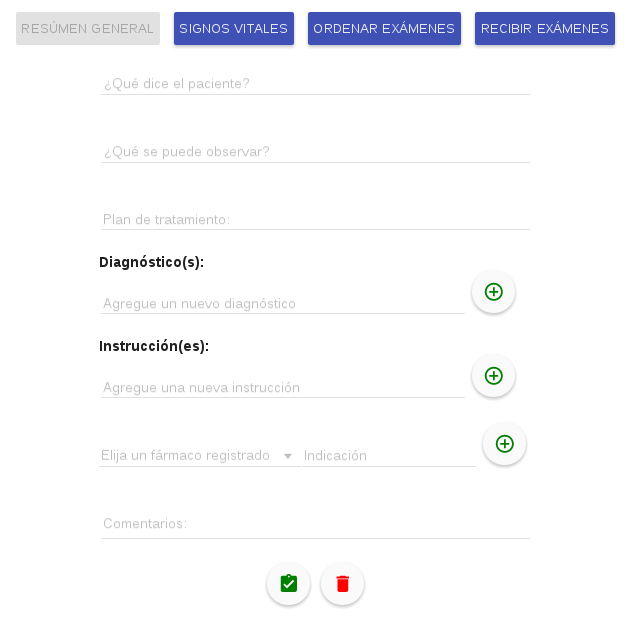
\includegraphics[width=.75\textwidth,keepaspectratio=true]{figures/consulta1}
                \end{center}
                \caption{Resumen General}
                \label{img-revisiongeneral}
            \end{figure}
                
        \item Signos Vitales (figura \ref{img-signovital}):\\
        Para el caso en que aplique, se tiene esta sección de la consulta donde se registran los signos vitales tomados en la misma. Se tomó el nombre de ``Signos Vitales" por convención aunque refiere a datos fisiológicos en general: altura, peso, presión arterial y cualquier otro que el doctor considere pertinente. Se deja una acción especial para añadir al sistema nuevos parámetros; esto con la finalidad de permitir flexibilidad y mejorar la eficiencia de la carga de datos.
            \begin{itemize}
                \item Flexibilidad: En caso de precisar un nuevo parámetro fisiológico, por no estar previamente contemplado, el doctor puede agregarlo haciendo uso de la opción ``Otro".
                \item Carga de Datos: Dado que los parámetros requeridos pueden ser diferentes entre las disciplinas médicas, se estaría desperdiciando espacio en la base de datos si se tomara un sólo formulario con todos los parámetros registrados. Tomando en cuenta eso, se decidió que el doctor está en potestad de hacer la revisión del paciente y añadir los ``Signos Vitales" que considere pertinentes y que hayan sido medidos durante la consulta; así pues, un mismo doctor puede realizar dos consultas a un mismo paciente y en una registrar la ``temperatura corporal" (por ejemplo) y en otra consulta registrar la ``tensión arterial".
            \end{itemize}
            
            \begin{figure}[htb!]
                \begin{center}
                    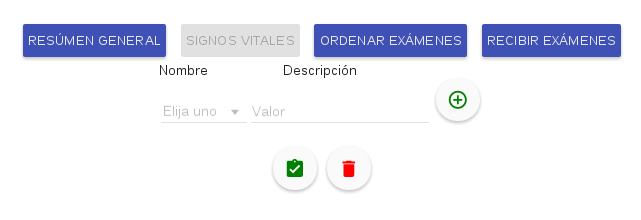
\includegraphics[width=.75\textwidth,keepaspectratio=true]{figures/consulta2}
                \end{center}
                \caption{Signos Vitales}
                \label{img-signovital}
            \end{figure}
        \item Solicitud de Examen Médico (figura \ref{img-solicitarexamen}):\\
        En este caso se utilizó un formulario dinámico para el registro de solicitud de exámenes médicos. En esta fase, el exámen sólo cuenta con un nombre, dado por el doctor tratante, y se registra la solicitud que puede ser recibida en una consulta futura en la sección ``Recibir Exámenes" descrita a continuación.
        
        \begin{figure}[htb!]
            \begin{center}
                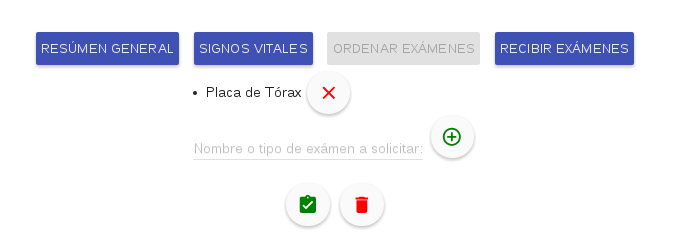
\includegraphics[width=.75\textwidth,keepaspectratio=true]{figures/consulta3}
            \end{center}
            \caption{Solicitud de Examen Médico}
            \label{img-solicitarexamen}
        \end{figure}
        
        \item Recepción de Examen Médico (figura \ref{img-recibirexamen}):\\
        En esta fase el doctor puede indicar la recepción de un examen médico solicitado en una consulta previa, y sólo de los solicitados en consultas previas, junto con la carga de un archivo asociado al examen (en caso de poseer un archivo digital). La intención es mantener la información médica que llevó a diagnósticos de tal forma que se puedan realizar revisiones a la misma y estudios de evolución de pacientes. Ver figura \ref{img-recibirexamen}.
        
        \begin{figure}[htb!]
            \begin{center}
                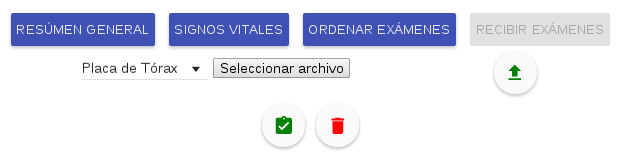
\includegraphics[width=.75\textwidth,keepaspectratio=true]{figures/consulta4}
            \end{center}
            \caption{Recepción de Examen Médico}
            \label{img-recibirexamen}
        \end{figure}
    \end{itemize}
    
    Para este Sprint, debido a la complejidad del formulario y la encapsulación de los datos requeridos, se asignó una duración de tres semanas en las cuales el equipo de desarrollo realizó la revisión de los tutoriales antes mencionados para lograr la correcta encapsulación de los datos.
    
    Para las pruebas de este Sprint se siguieron los siguientes parámetros:
    
    \begin{itemize}
        \item Respuestas y aceptación de UI.
        \item Encapsulación adecuada de los datos: Que los datos se preserven entre las distintas subvistas.
        \item Carga de datos en el sistema: Cantidad de datos y momento de transmisión.
        \item Formularios dinámicos y la respectiva carga de datos al formulario principal.
        \item Correctitud de los datos almacenados en el sistema.
    \end{itemize}
    
    Se dejó para el siguiente Sprint la revisión de la correcta carga de datos como la fecha para realizar la prueba conjunta con la revisión de la recuperación de datos de la vista \ref{historial-medico}.
    
    \subsection{Noveno Sprint: Vista de Historial de Consultas Médicas del Paciente}
    \label{historial-medico}
    
    En esta vista se presenta el historial completo de consultas médicas del paciente, ordenadas de manera cronológica y empezando por la última consulta. También se puede acceder a otros aspectos del historial médico, como por ejemplo hábitos, alergias, etc; tal y como se puede ver en la figura \ref{consultas}.
    
    \begin{figure}[htbp!]
        \begin{center}
            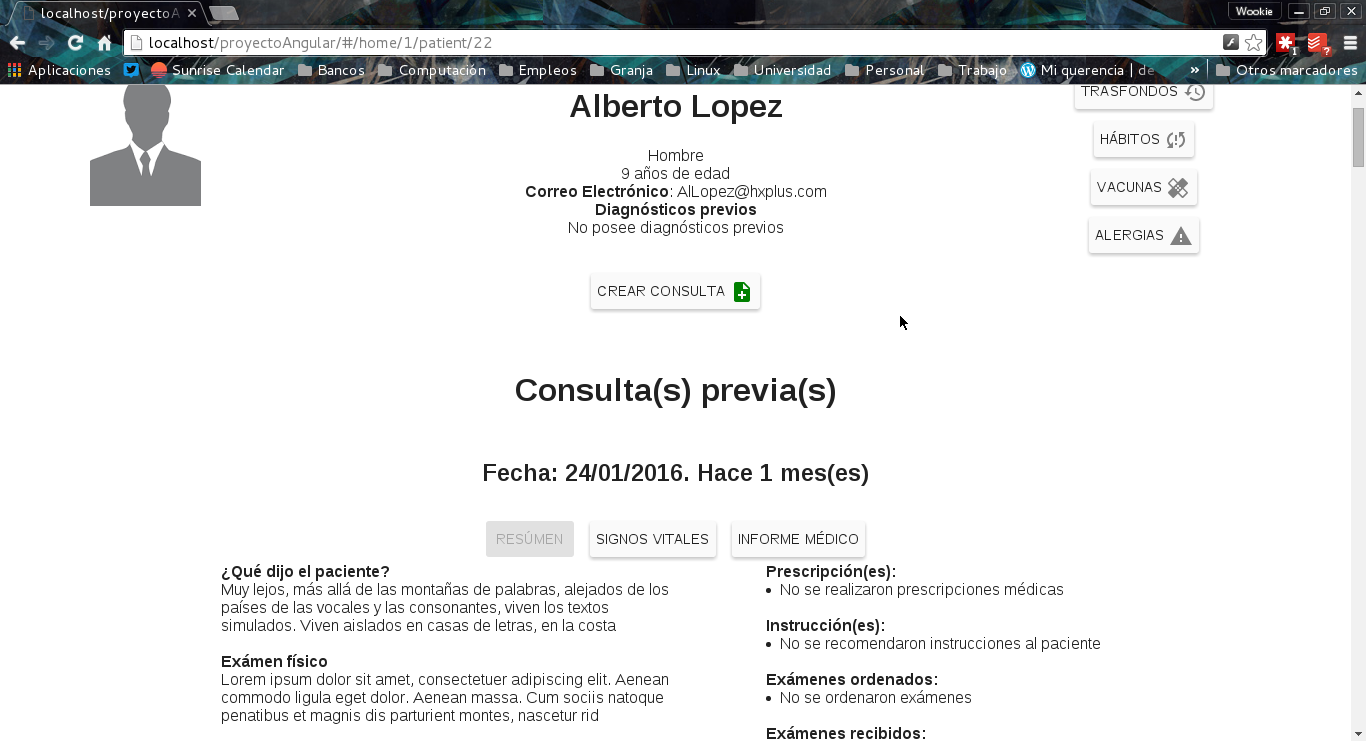
\includegraphics[width=.9\textwidth]{figures/p11}
        \end{center}
        \caption{Vista de Historial de Consultas Médicas del Paciente}
        \label{consultas}
    \end{figure}
    
    La vista permite a su vez la integración con la vista de Revisión de Consulta Médica (ver \ref{revisar-consulta}) y Agregar Consulta (ver \ref{crear-consulta}).
    
    Las pruebas para esta vista fueron principalmente de aceptación de UI pero se tomó en cuenta la agregación de nuevas consultas a la lista una vez realizada la consulta y almacenada en el sistema. Además se revisó la integración con la vista de agregar consulta médica (ver \ref{crear-consulta}) y las acciones que ella realiza dentro del sistema.
    
    Para este Sprint se asignaron dos semanas pero debido a problemas de integración con las vistas mencionadas, fue requerido una semana adicional de revisión para el correcto funcionamiento de la vista (figura \ref{consultas}).
    
    \subsection{Décimo Sprint: Vista de Revisión de Consulta Médica}
    \label{revisar-consulta}
    Esta vista está insertada en la vista anterior logrando que lo que se llama ``Historial Médico" de un paciente sea en sí la lista de todas las consultas médicas junto con los respectivos accesos a trasfondos, alergias, entre otros. La revisión de consulta médica se divide en dos fases:
    
    \begin{enumerate}
        \item Resumen\\
        Resumen general de la consulta, se muestra la \textit{Soap Note} de la consulta y los exámenes solicitados y recibidos con su respectivo archivo, según coresponda (figura \ref{consultarev-resumen}).
        \item Signos Vitales\\
        En esta subvista se muestran los signos vitales recabados durante la consulta. Se muestra un mensaje adecuado en caso de no haberse recabado signos vitales durante dicha consulta. Se hace en un apartado para no saturar la vista principal de ``Resumen" con lo que es información muy específica y potencialmente puede ser excesiva para una vista ya cargada (figura \ref{consultarev-signosv}).
    \end{enumerate}
    
    Para este Sprint se asignaron dos semanas y las pruebas fueron realizadas tomando en cuenta:
    
    \begin{itemize}
        \item Integración con la vista \ref{historial-medico}.
        \item Actualización de los datos y revisión de los mismos al momento de agregar una nueva consulta (vista \ref{crear-consulta}).
        \item Aceptación de UI.
    \end{itemize}
    
    \begin{figure}[htb!]
        \begin{center}
            \begin{minipage}{0.45\textwidth}
                \begin{center}
                    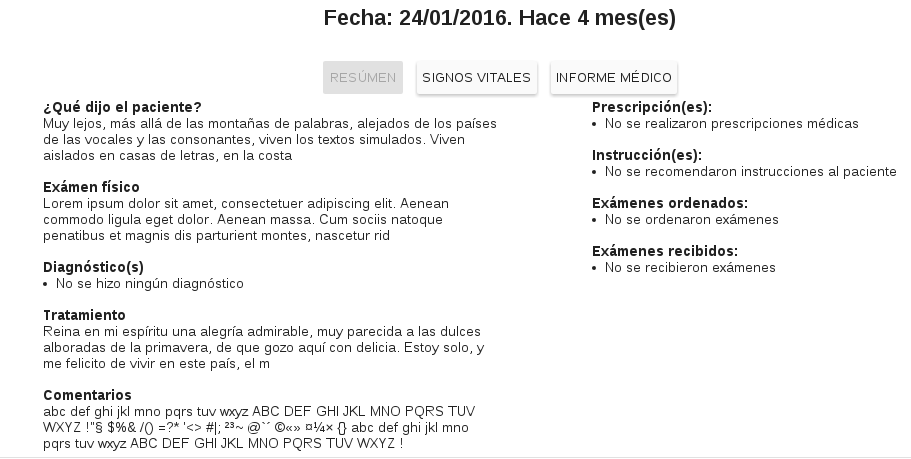
\includegraphics[width=\linewidth,keepaspectratio=true]{figures/consultarev-resumen}
                \end{center}
                \caption{Vista de Revisión de consulta. Resumen}
                \label{consultarev-resumen}
            \end{minipage}
            \hspace*{\fill}
            \begin{minipage}{0.45\textwidth}
                \begin{center}
                    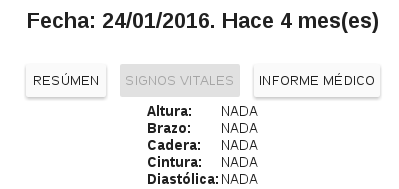
\includegraphics[width=\linewidth,keepaspectratio=true]{figures/consultarev-signosv}
                \end{center}
                \caption{Vista de Revisión de consulta. Signos Vitales}
                \label{consultarev-signosv}
            \end{minipage}
        \end{center}
    \end{figure}
    
    \subsection{Décimo Primer Sprint: Vista de Generación de Reportes Médicos}
    Esta vista se anexa a la ``Vista de Revisión de Consulta Méddica" como un apartado final. En ella el doctor puede generar un reporte con los datos de la consulta dada, seleccionando los que desea plasmar en dicho reporte, y descargar un archivo en formato PDF para ser entregado de manera digital o impreso directamente. También puede optar por generar un reposo médico, indicando la cantidad de días asignados a dicho reposo y descargando el archivo.
    
    En este punto el equipo de desarrollo precisó una semana de capacitación por la utilización de iText (ver punto \ref{tecno-itext}) herramienta que fue la elegida para la generación de archivos PDF y que hasta el momento no había sido utilizada en el desarrollo.
    
    Tomando en cuenta la semana de capacitación, este Sprint contó con una duración de dos semanas y las pruebas fueron basadas en:
    
    \begin{itemize}
        \item Aceptación de UI.
        \item Correctitud de la información en el informe médico generado(figuras \ref{reportes-informenav} y \ref{reportes-informepdf}).
        \item Correctitud de la información en los reposos médicos (figuras \ref{reportes-reposonav} y \ref{reportes-reposopdf}).
        \item Aceptación del formato visual de ambas clases de archivos.
    \end{itemize}
    %  Informe
    \begin{figure}[htb!]
        \begin{minipage}{0.45\textwidth}
            \begin{center}
                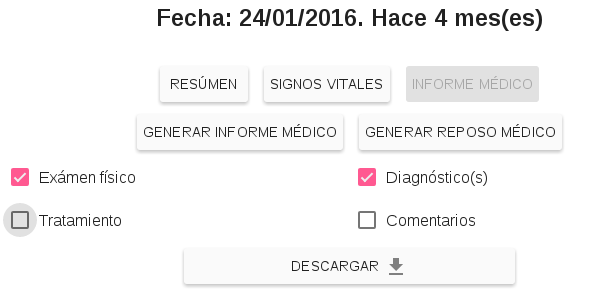
\includegraphics[width=\linewidth,keepaspectratio=true]{figures/reportes-informenav}
            \end{center}
            \caption{Vista de Generación de Reportes Médicos. Informe}
            \label{reportes-informenav}
        \end{minipage}
        \hspace*{\fill}
        \begin{minipage}{0.45\textwidth}
            \begin{center}
                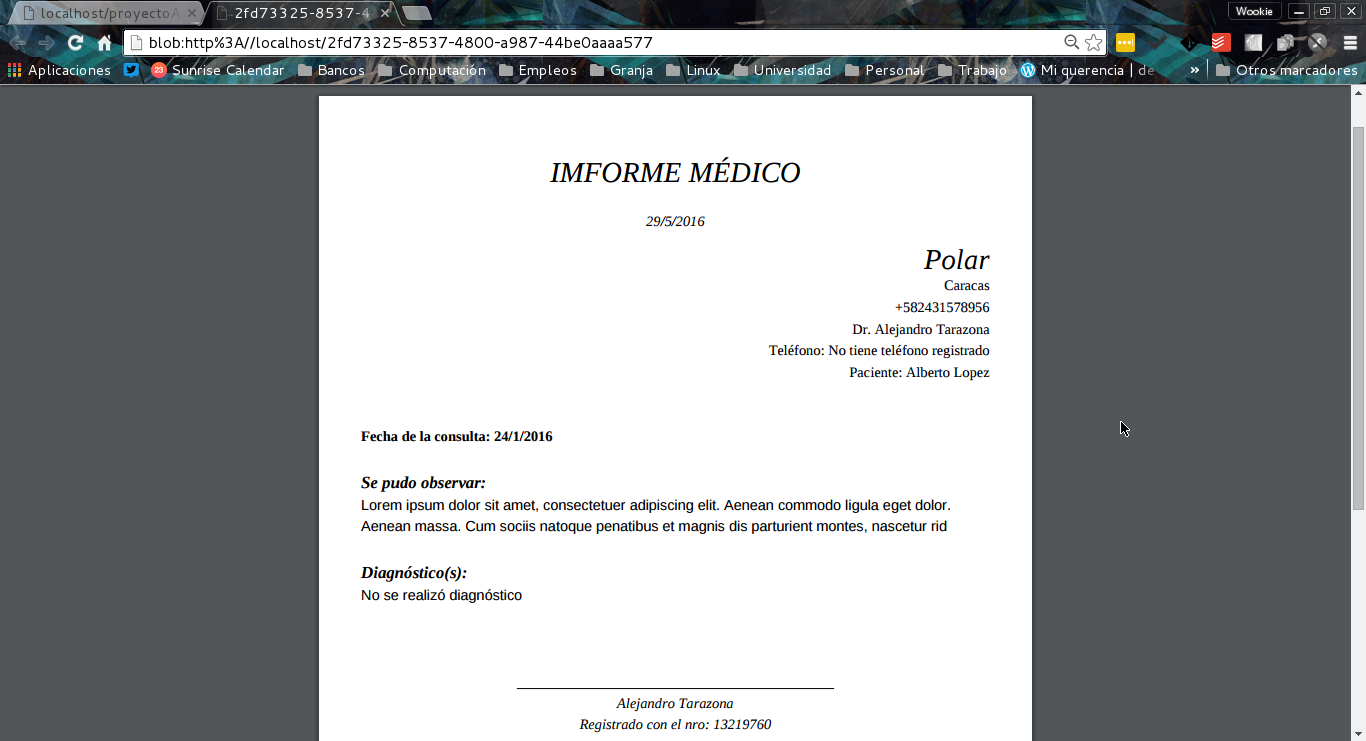
\includegraphics[width=\linewidth,keepaspectratio=true]{figures/reportes-informepdf}
            \end{center}
            \caption{Archivo de informe médico generado por el sistema}
            \label{reportes-informepdf}
        \end{minipage}
    \end{figure}
    
    %  Reposo
    \begin{figure}[htb!]
        \begin{minipage}{0.45\textwidth}
            \begin{center}
                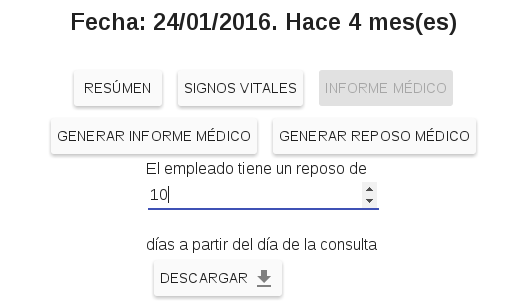
\includegraphics[width=\linewidth,keepaspectratio=true]{figures/reportes-reposonav}
            \end{center}
            \caption{Vista de Generación de Reportes Médicos. Reposo}
            \label{reportes-reposonav}
        \end{minipage}
        \hspace*{\fill}
        \begin{minipage}{0.45\textwidth}
            \begin{center}
                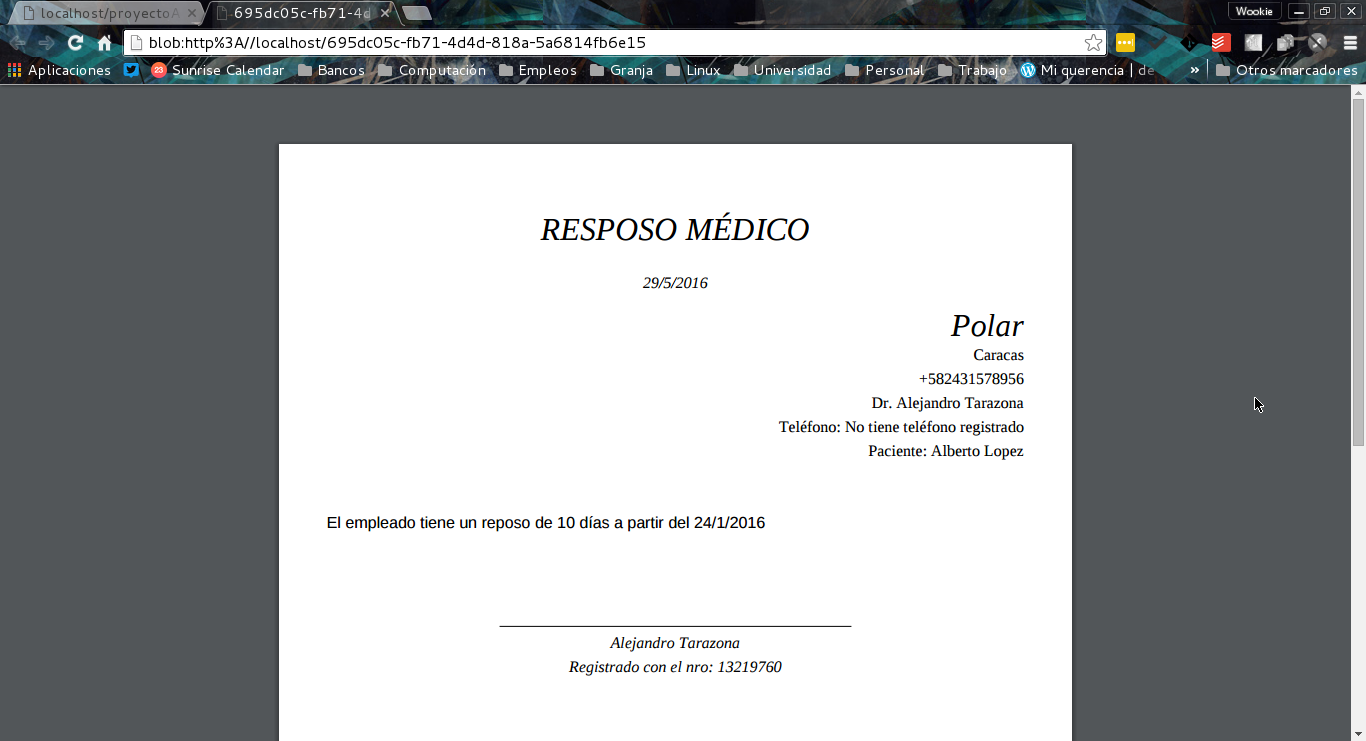
\includegraphics[width=\linewidth,keepaspectratio=true]{figures/reportes-reposopdf}
            \end{center}
            \caption{Archivo de reposo médico generado por el sistema}
            \label{reportes-reposopdf}
        \end{minipage}
    \end{figure}
    
    
\section{Fase de Cierre}

\subsection{Dificultades generales encontradas}

    Las dificultades encontradas durante el desarrollo del proyecto fueron:
    
    \begin{itemize}
        \item \textbf{Restricción en el uso de herramientas:} el \textit{Product Owner} solicitó explícitamente el uso de Java, SPRING, Hbernate, JavaScript, MySQL, AngularJS y JSON, tal y como fue descrito, para el desarrollo. Lo cual, si bien facilitó la creación y desarrollo del proyecto, dejó imposibilitada la posibilidad de, con tecnologías actuales, dar soporte a una base de datos orientada a eventos, tal como se pretendía hacer al principio.
        
        \item \textbf{Falta de informción de parte de Inpsasel:} originalmente se buscaba generar informes médicos especializados para el reporte de enfermedades ocupacionales al Inpsasel, órgano encargado de la gestión de enfermedades ocupacionales en el émbito nacional. Sin embargo, la falta de información, formatos y, más adelante, el lanzamiento de su portal (de Inpsasel) con automatización de dicha gestión, dejó a HxPlus Ocupacional sin la necesidad de realizar dichos informes.
    \end{itemize}
    
    \subsection{Resultados Generales}
    
    El proyecto de pasantía se completó satisfactoriamente. A pesar de no poseer la funcioncionalidad de generación de informes de Inpsasel, la empresa de consideró satisfecha con los módulos implementados. La línea de tiempo de consultas se muestra adecuadamente y en orden cronológico, los diagnósticos y planes son almacenados y mostrados a gusto de la empresa y de conformidad con los lineamientos.
    
    Queda de parte de la empresa gestionar el desarrollo de futuros módulos o funcionalidades para la aplicación.
        
     \chapter{Conclusiones y Recomendaciones}

    Habiendo terminado el proyecto, se logró la implementación del sistema ``HxPlus Ocupacional" para Globisoft S.A. apoyando de esta manera su misión de brindar apoyo tecnológico al área médica en Venezuela. El mercado actual de herramientas en este ámbito está en su fase inicial y, aunque hay resistencia al cambio por parte de los médicos nacionales, la familiaridad y una interfaz planificada para la usabilidad, ayudará a que las nuevas generaciones hagan uso de este sistema.
    
    SCRUM permitió una organización rápida y la debida evaluación oportuna de los objetivos logrados y la planificación de la siguiente serie de objetivos, adaptándose así a los inconvenientes evidenciados.
    
    El proyecto, si bien orientado a medicina ocupacional, se recomienda en un futuro, incluir también el área farmacéutica y su integración con ``HxPlus", el cual se encuentra en funcionamiento. Con esto se crearía un sistema distribuido integral de gestión de consultas, remisión de informes médicos y generación de constancias, informes y récipes médicos y que a su vez le permita a las empresas farmacéuticas publicidad y registros en tiempo real, a los pacientes, tener siempre a su disposición los planes de tratamiento, récipes médicos, los diagnósticos realizados y su historial médico en caso de alguna eventualidad como pérdida del mismo u olvidos ocasionales.
    
    También, y en el marco de las tecnologías usadas, se sugiere una evaluación del patrón de almacenamiento de la base de datos ya que el uso de un patrón orientado a eventos podría ser provechoso al momento de recuperación de fallos dentro de la base de datos.


    
     \addcontentsline{toc}{chapter}{Bibliografía}
\printbibliography
\pagebreak
     \addcontentsline{toc}{chapter}{Anexos}
\chapter*{Anexos}

\addcontentsline{toc}{section}{Anexo A: Diagrama ER-E y Glosario de términos}
\section*{Anexo A: Diagrama ER-E y Glosario de términos}
            \begin{figure}
                \begin{center}
                    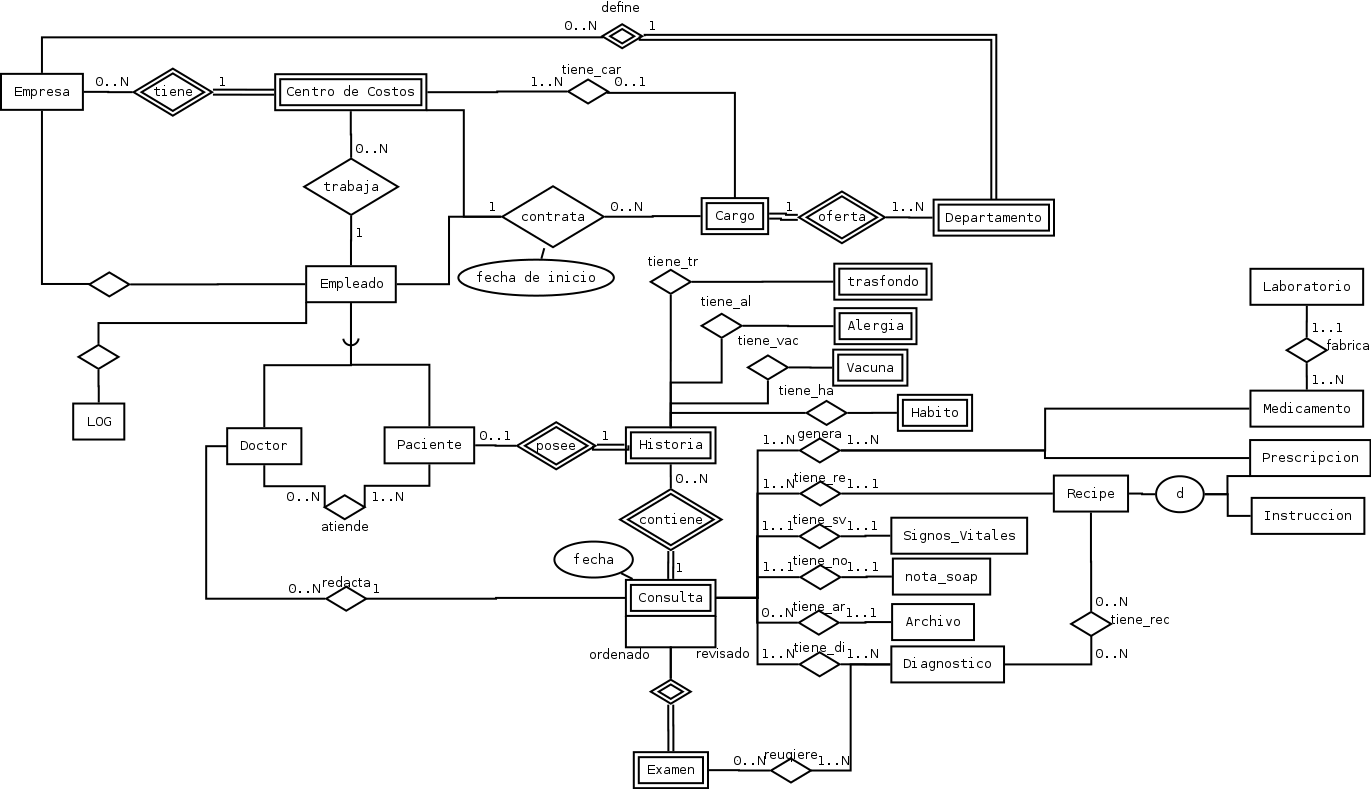
\includegraphics[scale=.45,angle=90]{figures/DiagramBD}
                \end{center}
                \caption{Diagrama ER-E de la base de datos.}
            \end{figure}

\pagebreak
    % Diagrama CU
    % Diagrama Clases
    % Diagrama ER-E <----Listo
    % Screenshots
    % DAS(?)
     
\end{document}